\documentclass[12pt,a4paper]{report}

\usepackage{iftex}
\ifPDFTeX
  \usepackage[utf8]{inputenc}
  \usepackage[T5]{fontenc}
  \usepackage{lmodern}
\else
  \usepackage{fontspec}
  \defaultfontfeatures{Ligatures=TeX}
  \IfFontExistsTF{Times New Roman}{
    \setmainfont{Times New Roman}
  }{
    \IfFontExistsTF{TeX Gyre Termes}{
      \setmainfont{TeX Gyre Termes}
    }{
      \setmainfont{Liberation Serif}
    }
  }
\fi
\usepackage[english,vietnamese]{babel}
\usepackage[a4paper,left=3cm,right=2cm,top=2cm,bottom=2cm]{geometry}
\usepackage{graphicx}
\usepackage{pdflscape}
\usepackage{tikz}
\usetikzlibrary{calc}
\usepackage{array}
\usepackage{booktabs}
\usepackage{longtable}
\usepackage{tabularx}
\usepackage{multirow}
\usepackage{setspace}
\usepackage{indentfirst}
\usepackage{float}
\usepackage[hyphens]{url}
\usepackage{xurl}
\usepackage{hyperref}
\usepackage{caption}
\usepackage{subcaption}
\usepackage{enumitem}
\usepackage{verbatim}

\hypersetup{
  hidelinks,
  pdfauthor={Nguyễn Nhật Hồng Phước},
  pdftitle={Xây dựng ứng dụng hỗ trợ quét đơn thuốc và lập kế hoạch dùng thuốc},
  pdfsubject={Báo cáo ngành Khoa học máy tính}
}

\makeatletter
\renewcommand\normalsize{%
  \@setfontsize\normalsize{13pt}{15.6pt}%
  \abovedisplayskip 12pt plus 3pt minus 7pt%
  \abovedisplayshortskip \z@ plus 3pt%
  \belowdisplayshortskip 7pt plus 3pt minus 4pt%
  \belowdisplayskip \abovedisplayskip
  \let\@listi\@listI
}
\makeatother
\normalsize
\setstretch{1.2}
\setlength{\parindent}{1cm}
\setlength{\parskip}{0pt}
\setcounter{secnumdepth}{3}
\setcounter{tocdepth}{2}
\setlength{\emergencystretch}{4em}
\setlength{\tabcolsep}{6pt}
\setlength{\extrarowheight}{3pt}
\setlength{\arrayrulewidth}{0.6pt}
\renewcommand{\arraystretch}{1.25}
\renewcommand{\tabularxcolumn}[1]{m{#1}}
\setcounter{topnumber}{3}
\setcounter{bottomnumber}{2}
\setcounter{totalnumber}{5}
\renewcommand{\topfraction}{0.9}
\renewcommand{\bottomfraction}{0.8}
\renewcommand{\textfraction}{0.07}
\renewcommand{\floatpagefraction}{0.8}

\addto\captionsvietnamese{%
  \renewcommand{\contentsname}{MỤC LỤC}%
  \renewcommand{\listfigurename}{DANH MỤC HÌNH ẢNH}%
  \renewcommand{\listtablename}{DANH MỤC BẢNG BIỂU}%
  \renewcommand{\bibname}{TÀI LIỆU THAM KHẢO}%
}
\renewcommand{\chaptername}{Chương}
\renewcommand{\tablename}{Bảng}
\renewcommand{\figurename}{Hình}

\captionsetup{font=normalsize,labelfont=bf}
\captionsetup[table]{position=above,justification=raggedright,singlelinecheck=false,skip=4pt}
\captionsetup[figure]{justification=centering}
\Urlmuskip=0mu plus 1mu\relax

% Fixed full-grid table templates modeled after the reference thesis.
% Every template draws both vertical and horizontal borders for all rows.
% J: standard 3-column table (STT / title / description)
% K: standard 4-column table (STT / group / example / role)
% Q: entity-detail table (STT / field / type / description / key)
% N: benchmark table (STT / metric / right-aligned value)
\newcolumntype{J}{|C{1.2cm}|L{4.4cm}|Y|}
\newcolumntype{K}{|C{1.0cm}|L{3.2cm}|L{3.9cm}|Y|}
\newcolumntype{Q}{|C{0.9cm}|L{2.8cm}|C{2.8cm}|Y|C{1.9cm}|}
\newcolumntype{N}{|C{1.2cm}|Y|R{3.0cm}|}
\newcommand{\TableHeader}[1]{\hline #1 \\ \hline}
\newcommand{\TableRow}[1]{#1 \\ \hline}

\makeatletter
\def\@makechapterhead#1{%
  \vspace*{8\p@}%
  {\parindent \z@ \centering \normalfont
    \ifnum \c@secnumdepth >\m@ne
      \LARGE\bfseries \MakeUppercase{\chaptername\ \thechapter}\par\nobreak
      \vskip 12\p@
    \fi
    \LARGE\bfseries
    \parbox{0.92\textwidth}{\centering #1}\par\nobreak
    \vskip 28\p@
  }}
\def\@makeschapterhead#1{%
  \vspace*{8\p@}%
  {\parindent \z@ \centering \normalfont
    \LARGE\bfseries
    \parbox{0.92\textwidth}{\centering #1}\par\nobreak
    \vskip 28\p@
  }}
\makeatother

\pagestyle{plain}

\newcolumntype{L}[1]{>{\raggedright\arraybackslash}m{#1}}
\newcolumntype{C}[1]{>{\centering\arraybackslash}m{#1}}
\newcolumntype{R}[1]{>{\raggedleft\arraybackslash}m{#1}}
\newcolumntype{Y}{>{\raggedright\arraybackslash}X}
\newcolumntype{M}{>{\centering\arraybackslash}X}
\newcolumntype{Z}{>{\raggedleft\arraybackslash}X}

\newcommand{\daihoc}{ĐẠI HỌC CẦN THƠ}
\newcommand{\truong}{TRƯỜNG CÔNG NGHỆ THÔNG TIN VÀ TRUYỀN THÔNG}
\newcommand{\loaibaocao}{\shortstack[c]{BÁO CÁO NIÊN LUẬN\\NGÀNH KHOA HỌC MÁY TÍNH}}
\newcommand{\tentailieu}{\shortstack[c]{XÂY DỰNG ỨNG DỤNG HỖ TRỢ\\QUÉT ĐƠN THUỐC VÀ\\LẬP KẾ HOẠCH DÙNG THUỐC}}
\newcommand{\tentailieuen}{\shortstack[c]{BUILDING A MOBILE APPLICATION\\FOR PRESCRIPTION SCANNING\\AND MEDICATION PLANNING}}
\newcommand{\sinhvien}{Nguyễn Nhật Hồng Phước}
\newcommand{\mssv}{B2308385}
\newcommand{\gvhd}{TS.\ Lưu Tiến Đạo}
\newcommand{\nganh}{Khoa học máy tính}
\newcommand{\thoigian}{Cần Thơ, tháng 4 năm 2026}

\newcommand{\drawcoverframe}{%
  \begin{tikzpicture}[remember picture,overlay]
    \draw[line width=2.2pt]($(current page.north west)+(1.5cm,-1.5cm)$) rectangle ($(current page.south east)+(-1.5cm,1.5cm)$);
    \draw[line width=0.8pt]($(current page.north west)+(1.65cm,-1.65cm)$) rectangle ($(current page.south east)+(-1.65cm,1.65cm)$);
  \end{tikzpicture}%
}

\begin{document}
\selectlanguage{vietnamese}
\hypersetup{pageanchor=false}

\begin{titlepage}
\thispagestyle{empty}
\newgeometry{left=2cm,right=2cm,top=2cm,bottom=2cm}
\drawcoverframe
\begin{center}
    \textbf{BỘ GIÁO DỤC VÀ ĐÀO TẠO}\\[0.2cm]
    \textbf{\daihoc}\\[0.2cm]
    \textbf{\truong}\\[1.2cm]

    
\includegraphics[width=2.9cm]{assets/ctu-logo.png}\\[1.0cm]

    {\Large \bfseries \loaibaocao}\\[1.2cm]

    {\normalsize \bfseries \tentailieu}\\[1.5cm]
    {\normalsize \bfseries \tentailieuen}\\[1.4cm]

    Sinh viên thực hiện: \textbf{\sinhvien} \\[0.25cm]
    Mã số sinh viên: \textbf{\mssv} \\[0.25cm]
    Ngành: \textbf{\nganh} \\[0.25cm]
    Giáo viên hướng dẫn: \textbf{\gvhd}

    \vfill
    \textbf{\thoigian}
\end{center}
\end{titlepage}

\restoregeometry

\begin{titlepage}
\thispagestyle{empty}
\drawcoverframe
\begin{center}
    \textbf{BỘ GIÁO DỤC VÀ ĐÀO TẠO}\\[0.2cm]
    \textbf{\daihoc}\\[0.2cm]
    \textbf{\truong}\\[1.0cm]

    
\includegraphics[width=2.7cm]{assets/ctu-logo.png}\\[0.9cm]

    {\Large \bfseries \loaibaocao}\\[1.0cm]
    {\normalsize \bfseries \tentailieu}\\[1.3cm]
    {\normalsize \bfseries \tentailieuen}\\[1.2cm]

    \begin{tabular}{rl}
        Sinh viên thực hiện: & \textbf{\sinhvien} \\
        Mã số sinh viên: & \textbf{\mssv} \\
        Giáo viên hướng dẫn: & \textbf{\gvhd} \\
    \end{tabular}

    \vfill
    \textbf{\thoigian}
\end{center}
\end{titlepage}

\hypersetup{pageanchor=true}

\pagenumbering{roman}

\chapter*{LỜI CAM ĐOAN}
\addcontentsline{toc}{chapter}{LỜI CAM ĐOAN}

Tôi xin cam đoan báo cáo này là kết quả nghiên cứu, thiết kế, cài đặt và tổng hợp của cá nhân tôi dưới sự hướng dẫn của \gvhd. Các nội dung mô tả trong báo cáo được xây dựng dựa trên quá trình phát triển hệ thống hỗ trợ quét đơn thuốc và lập kế hoạch dùng thuốc, trên kết quả thử nghiệm thực tế của dự án, cùng với các tài liệu tham khảo đã được trích dẫn rõ ràng. Tôi xin chịu trách nhiệm về tính trung thực của các số liệu, nhận xét và kết luận được trình bày trong báo cáo.

\chapter*{LỜI CẢM ƠN}
\addcontentsline{toc}{chapter}{LỜI CẢM ƠN}

Trong quá trình thực hiện đề tài, tôi đã nhận được nhiều sự hỗ trợ quý báu từ giảng viên hướng dẫn, bạn bè và những người thân xung quanh. Tôi xin gửi lời cảm ơn chân thành đến \gvhd{} đã định hướng chuyên môn, góp ý về cách tiếp cận bài toán và giúp tôi điều chỉnh phạm vi thực hiện theo hướng phù hợp với điều kiện thời gian cũng như mục tiêu học thuật của đề tài.

Tôi cũng xin cảm ơn các thầy cô của Trường Công nghệ Thông tin và Truyền thông, Đại học Cần Thơ đã trang bị cho tôi nền tảng kiến thức trong suốt quá trình học tập. Bên cạnh đó, tôi xin cảm ơn gia đình và bạn bè đã luôn động viên, hỗ trợ tôi trong quá trình hoàn thiện hệ thống, kiểm thử ứng dụng và hoàn thành báo cáo này.

Mặc dù đã cố gắng hoàn thiện báo cáo ở mức tốt nhất, đề tài chắc chắn vẫn còn những thiếu sót. Tôi rất mong nhận được thêm các ý kiến đóng góp để tiếp tục hoàn thiện sản phẩm và mở rộng nghiên cứu trong tương lai.

\tableofcontents
\clearpage
\listoffigures
\clearpage
\listoftables
\clearpage

\chapter*{DANH MỤC TỪ VIẾT TẮT}
\addcontentsline{toc}{chapter}{DANH MỤC TỪ VIẾT TẮT}

{\renewcommand{\arraystretch}{1.4}
\noindent
\begin{tabularx}{\textwidth}{J}
\TableHeader{\textbf{STT} & \textbf{Từ viết tắt} & \textbf{Diễn giải}}
\TableRow{1 & AI & Trí tuệ nhân tạo}
\TableRow{2 & API & Giao diện lập trình ứng dụng}
\TableRow{3 & CNN & Mạng nơ-ron tích chập}
\TableRow{4 & ERD & Sơ đồ thực thể - liên kết}
\TableRow{5 & GPU & Bộ xử lý đồ họa}
\TableRow{6 & JSON & Định dạng dữ liệu JSON}
\TableRow{7 & NER & Nhận dạng thực thể tên}
\TableRow{8 & OCR & Nhận dạng ký tự quang học}
\TableRow{9 & REST & Kiểu giao tiếp dữ liệu REST}
\TableRow{11 & YOLO & Thuật toán phát hiện đối tượng thời gian thực YOLO}
\end{tabularx}}

\clearpage
\chapter*{ABSTRACT}
\addcontentsline{toc}{chapter}{ABSTRACT}
\selectlanguage{english}

This report presents the design and implementation of a system that supports prescription scanning and medication plan creation by combining optical character recognition and artificial intelligence techniques. The system is organized into three components: a mobile application for user interaction, a Node.js server for business logic and data management, and an AI service for prescription-region detection, image preprocessing, OCR, sequential line-order grouping, drug-name extraction, and drug-database matching.

Experimental results on a dataset of 50 real-world prescription images demonstrate that the system successfully processed 100\% of the cases, extracting 338 drug items with an average of about 6.8 drugs per image. These findings initially affirm the feasibility and effectiveness of the proposed architecture in digitizing prescription data.

The report also acknowledges several current limitations. At this stage, the model mainly focuses on recognizing the drug list rather than the entire prescription content, so further in-depth research and evaluation are still needed.

\noindent\textbf{Keywords:} prescription, optical character recognition, drug name extraction, mobile application, medication plan, drug recognition.

\clearpage
\selectlanguage{vietnamese}
\chapter*{TÓM TẮT}
\addcontentsline{toc}{chapter}{TÓM TẮT}

Báo cáo này trình bày quá trình thiết kế và xây dựng một hệ thống hỗ trợ quét đơn thuốc và lập kế hoạch dùng thuốc, bằng cách sử dụng nhận dạng ký tự quang học (OCR) và mô hình ngôn ngữ trung bình (PhoBert) kết hợp với các công nghệ như Flutter và Node.js. Bài toán xuất phát từ nhu cầu thực tiễn của người bệnh, đặc biệt là những người lớn tuổi hoặc gặp khó khăn trong việc đọc và ghi nhớ thông tin từ đơn thuốc giấy để tự lập lịch uống thuốc hằng ngày. Mục tiêu trọng tâm là chuyển đổi thông tin trên ảnh đơn thuốc thành một kế hoạch, qua đó giúp người dùng dễ dàng rà soát và sử dụng thuốc.

Về kiến trúc, hệ thống được tổ chức thành ba thành phần tách biệt: ứng dụng di động phụ trách giao diện người dùng, máy chủ Node.js quản lý dữ liệu và nghiệp vụ, mô-đun AI thực hiện chuỗi xử lý gồm phát hiện vùng đơn thuốc, tiền xử lý ảnh, OCR, gom các khối theo số thứ tự dòng thuốc, trích xuất tên thuốc và đối sánh cơ sở dữ liệu thuốc.

Kết quả thực nghiệm trên tập dữ liệu gồm 50 ảnh đơn thuốc thực tế cho thấy hệ thống xử lý thành công 100\% trường hợp, trích xuất được 338 mục thuốc với trung bình khoảng 6,8 thuốc trên mỗi ảnh. Những kết quả này bước đầu khẳng định tính khả thi và hiệu quả của kiến trúc đề xuất trong việc số hóa dữ liệu đơn thuốc. Bên cạnh đó, báo cáo cũng nhìn nhận khách quan một số giới hạn hiện tại, như việc mô hình mới tập trung nhận diện phần danh sách thuốc thay vì toàn bộ nội dung đơn, cần được nghiên cứu, đánh giá sâu hơn trong tương lai.

\noindent\textbf{Từ khóa:} đơn thuốc, nhận dạng ký tự quang học, trích xuất tên thuốc, ứng dụng di động, kế hoạch dùng thuốc, nhận diện thuốc.

\clearpage
\pagenumbering{arabic}

\chapter{GIỚI THIỆU}

\section{Đặt vấn đề}

Trong thực tế chăm sóc sức khỏe cá nhân, đơn thuốc giấy vẫn là hình thức phổ biến tại nhiều cơ sở y tế. Tuy nhiên, việc chuyển thông tin từ đơn thuốc giấy sang một hình thức dễ theo dõi hơn vẫn còn phụ thuộc nhiều vào thao tác thủ công của người bệnh hoặc người nhà. Người dùng phải đọc lại tên thuốc, tự nhập tên thuốc vào điện thoại hoặc ghi chú ra giấy, sau đó tự nhớ giờ uống và số lần uống trong ngày. Quy trình này vừa tốn thời gian, vừa dễ xảy ra sai sót, đặc biệt đối với người lớn tuổi hoặc người không quen sử dụng ứng dụng số.

Trong bối cảnh đó, việc xây dựng một hệ thống có thể hỗ trợ quét đơn thuốc, nhận diện tên thuốc và chuyển trực tiếp thành kế hoạch dùng thuốc là một hướng tiếp cận có giá trị thực tế cao. Khó khăn lớn nhất của bài toán nằm ở việc đơn thuốc thực tế có bố cục không đồng nhất, chất lượng ảnh chụp thay đổi mạnh, chữ in trên giấy có thể bị nghiêng, mờ, chói hoặc thiếu vùng nội dung. Do đó, hệ thống cần đồng thời giải quyết bài toán xử lý ảnh, OCR, trích xuất thông tin thuốc và thiết kế ứng dụng sao cho người dùng cuối vẫn có thể thao tác dễ dàng.

\section{Mục tiêu đề tài}

Mục tiêu tổng quát của đề tài là xây dựng một hệ thống hỗ trợ quản lý dùng thuốc từ đơn thuốc giấy, trong đó trí tuệ nhân tạo đóng vai trò hỗ trợ nhận diện thông tin thuốc còn ứng dụng di động đóng vai trò đưa công nghệ này vào một luồng sử dụng thực tế.

Các mục tiêu cụ thể gồm:

\begin{enumerate}[label=\arabic*.]
    \item Xây dựng quy trình nhận diện đơn thuốc từ ảnh đầu vào để trích xuất danh sách thuốc phục vụ cho các bước xử lý tiếp theo.
    \item Xây dựng máy chủ trung gian để kết nối ứng dụng di động với mô-đun AI, đồng thời quản lý dữ liệu lịch sử quét, kế hoạch dùng thuốc và nhật ký uống thuốc.
    \item Xây dựng ứng dụng di động cho phép người dùng quét đơn thuốc, rà soát lại kết quả, thiết lập giờ uống và theo dõi việc dùng thuốc theo ngày.
    \item Đánh giá những hướng mở rộng đã được cân nhắc nhưng chưa nên đưa vào phiên bản chính, chẳng hạn như mở rộng nhận dạng ký tự quang học sang các vùng thông tin khác trên đơn hoặc xác minh viên thuốc qua hình ảnh.
\end{enumerate}

\section{Ý nghĩa thực tiễn của đề tài}

Đề tài có ý nghĩa thực tiễn ở chỗ giúp giảm thao tác nhập tay thông tin thuốc từ đơn giấy, hỗ trợ người dùng thiết lập lịch uống rõ ràng hơn và thuận tiện hơn trong quá trình theo dõi việc dùng thuốc hằng ngày. Đối với người lớn tuổi hoặc người chăm sóc, một ứng dụng có thể quét đơn, gợi ý danh sách thuốc và hỗ trợ lập lịch sẽ dễ sử dụng hơn so với cách ghi nhớ hoặc ghi chép thủ công.

\section{Đối tượng nghiên cứu}

Đối tượng nghiên cứu của đề tài là ảnh đơn thuốc giấy, thông tin thuốc cần trích xuất từ ảnh và luồng tạo kế hoạch dùng thuốc trên ứng dụng di động. Đề tài tập trung vào phần thông tin liên quan trực tiếp đến thuốc và bước lập lịch, không đặt trọng tâm vào việc trích xuất toàn bộ nội dung hành chính hoặc chẩn đoán trên đơn thuốc.

\section{Phạm vi thực hiện}

Đề tài tập trung vào luồng chính của sản phẩm gồm: quét đơn thuốc, nhận diện danh sách thuốc, xác nhận kết quả nhận diện, lập lịch dùng thuốc, lưu kế hoạch và hỗ trợ theo dõi việc uống thuốc. Đây là phần có tính khả dụng thực tế cao nhất trong phạm vi đề tài và cũng là phần đã được hoàn thiện ở mức đầu cuối.

Về nội dung trích xuất, hệ thống ưu tiên các thông tin phục vụ trực tiếp cho bài toán lập lịch dùng thuốc, đặc biệt là tên thuốc và các tín hiệu liên quan đến danh sách thuốc. Mặc dù về mặt kỹ thuật có thể mở rộng nhận dạng ký tự quang học để lấy thêm họ tên bệnh nhân, triệu chứng hoặc chẩn đoán, phạm vi đó chưa được đưa vào phiên bản chính vì làm tăng thời gian xử lý và yêu cầu điều kiện chụp ảnh nghiêm ngặt hơn.

Một hướng khác cũng đã được khảo sát là chức năng xác minh viên thuốc qua hình ảnh. Dự án hiện đã có một số màn hình thử nghiệm cho hướng này, nhưng chức năng đó chưa được xem là một phần của luồng chính đã được kiểm chứng trong đề tài vì vẫn còn rủi ro an toàn nếu hệ thống nhận nhầm các viên thuốc có ngoại hình gần giống nhau. Nội dung này được phân tích như một giới hạn và hướng phát triển ở các chương sau.

\section{Phương pháp nghiên cứu}

Đề tài được triển khai theo hướng kết hợp giữa nghiên cứu ứng dụng và phát triển hệ thống. Thay vì chỉ dừng lại ở việc thử nghiệm một mô hình OCR hoặc một mô hình nhận diện đơn lẻ, hệ thống được thiết kế thành ba phần rõ ràng: ứng dụng di động, máy chủ và mô-đun AI. Cách làm này giúp kiểm tra tính khả thi của một sản phẩm hoàn chỉnh trong bối cảnh sử dụng thực tế, đồng thời thuận lợi hơn cho việc đánh giá từng phần của hệ thống.

Quá trình nghiên cứu và triển khai được thực hiện theo các bước chính sau:

\begin{enumerate}[label=\arabic*.]
    \item Nghiên cứu tài liệu về nhận dạng ký tự quang học, trích xuất tên thuốc và thiết kế ứng dụng hỗ trợ dùng thuốc.
    \item Phân tích bài toán thực tế và xác định phạm vi ưu tiên cho luồng quét đơn thuốc, rà soát kết quả và lập lịch dùng thuốc.
    \item Thiết kế kiến trúc hệ thống gồm ứng dụng di động, máy chủ, mô-đun AI và cơ sở dữ liệu.
    \item Cài đặt, kết nối và kiểm thử từng thành phần trước khi đánh giá luồng hoạt động đầu cuối.
    \item Tổng hợp kết quả, phân tích hạn chế và đề xuất các hướng phát triển tiếp theo.
\end{enumerate}

Về kỹ thuật, quy trình xử lý quét đơn thuốc được tổ chức theo chuỗi: phát hiện vùng đơn thuốc, tiền xử lý ảnh, kiểm tra chất lượng, OCR, gom khối OCR theo số thứ tự, trích xuất tên thuốc và chuẩn hóa tên thuốc. Ở phía ứng dụng, kết quả nhận diện luôn đi qua bước rà soát lại trước khi lập lịch nhằm giảm rủi ro sai sót trong ngữ cảnh y tế.

\section{Đóng góp của đề tài}

Các đóng góp chính của đề tài có thể tóm tắt như sau:

\begin{itemize}[leftmargin=1.5cm]
    \item Xây dựng được một hệ thống có luồng hoạt động đầu cuối từ ảnh đơn thuốc đến kế hoạch dùng thuốc trên ứng dụng di động.
    \item Kết hợp được nhiều thành phần trong cùng một quy trình xử lý gồm phát hiện vùng đơn thuốc, nhận dạng ký tự quang học, trích xuất thực thể tên thuốc và đối sánh cơ sở dữ liệu thuốc.
    \item Thiết kế máy chủ và mô hình dữ liệu đủ để quản lý kế hoạch dùng thuốc, lịch sử quét và nhật ký xác nhận liều uống.
    \item Phân tích trung thực các nội dung chưa nên tích hợp, đặc biệt là mở rộng nhận dạng ký tự quang học cho toàn bộ đơn thuốc và xác minh viên thuốc qua hình ảnh trong bối cảnh yêu cầu an toàn thực tế.
\end{itemize}

\section{Cấu trúc báo cáo}

Báo cáo gồm sáu chương. Chương 1 trình bày bối cảnh, mục tiêu, ý nghĩa thực tiễn, phạm vi và phương pháp nghiên cứu. Chương 2 trình bày cơ sở lý thuyết và công nghệ sử dụng. Chương 3 phân tích yêu cầu và thiết kế kiến trúc hệ thống. Chương 4 mô tả việc cài đặt từng thành phần chính của hệ thống. Chương 5 trình bày kết quả thực nghiệm, đánh giá và các giới hạn kỹ thuật. Chương 6 đưa ra kết luận và định hướng phát triển trong tương lai.

\chapter{CƠ SỞ LÝ THUYẾT VÀ CÔNG NGHỆ LIÊN QUAN}

\section{Bài toán nhận diện thông tin từ đơn thuốc}

Đơn thuốc là một dạng tài liệu bán cấu trúc. Mặc dù về tổng thể có những vùng thông tin thường gặp như thông tin bệnh nhân, thông tin bác sĩ, chẩn đoán và danh sách thuốc, cách trình bày giữa các mẫu đơn vẫn khác nhau. Ngoài ra, ảnh đơn thuốc trong điều kiện thực tế thường chịu ảnh hưởng bởi góc chụp, ánh sáng, bóng đổ, độ nghiêng, độ mờ và nền cảnh xung quanh. Vì vậy, hệ thống không thể coi ảnh đầu vào là một tài liệu phẳng và sạch như trong các bộ dữ liệu OCR chuẩn hóa.

Để làm rõ thách thức này, Hình~\ref{fig:real-prescription} minh họa một đơn thuốc thực tế được đưa vào hệ thống trong quá trình thử nghiệm. Trước khi đưa vào tài liệu, các thông tin hành chính cá nhân nhạy cảm của người bệnh đã được che đi nhằm đảm bảo an toàn quyền riêng tư. Có thể thấy, ảnh mang đặc trưng thực tế rất cao khi chịu tác động của góc chụp, độ cong của mặt giấy và điều kiện ánh sáng tự nhiên.

\begin{figure}[tbp]
\centering
\includegraphics[width=0.65\textwidth]{assets/real_data/donthuoc.pdf}
\caption{Ảnh đơn thuốc thực tế làm đầu vào của hệ thống (đã che thông tin cá nhân)}
\label{fig:real-prescription}
\end{figure}

Chính vì sự phức tạp của ảnh thực tế, một hệ thống chuyên dụng cần có khả năng tiền xử lý mạnh mẽ thay vì đưa ngay qua mô hình nhận diện văn bản. Với bài toán của đề tài, thông tin có giá trị nhất cần lấy ra là danh sách thuốc. Từ góc nhìn sản phẩm, đây là phần trực tiếp tạo ra giá trị cho người dùng vì danh sách thuốc là đầu vào để tạo kế hoạch dùng thuốc. Chính vì vậy, đề tài không theo đuổi chiến lược trích xuất toàn bộ nội dung trên đơn thuốc ngay từ đầu mà ưu tiên vùng thông tin đem lại tác dụng cao nhất cho luồng chính.

\section{Phát hiện đối tượng và cắt vùng đơn thuốc}

Trước khi áp dụng OCR, ảnh đầu vào cần được xác định và cắt ra vùng chứa nội dung đơn thuốc. Đây là bước quan trọng vì ảnh chụp thực tế thường bao gồm cả nền ảnh, tay người cầm đơn hoặc các vật thể xung quanh không liên quan. Nếu đưa toàn bộ ảnh vào OCR mà không qua bước này, chất lượng nhận dạng có thể giảm đáng kể do nhiễu từ nền và các vùng không phải văn bản.

Hệ thống sử dụng YOLO (You Only Look Once) cho bước phát hiện và cắt vùng đơn thuốc \cite{yolo}. YOLO là một thuật toán phát hiện đối tượng theo thời gian thực, được thiết kế để xử lý toàn bộ ảnh chỉ trong một lần suy luận duy nhất thay vì chia nhỏ ảnh thành nhiều vùng rồi xử lý từng vùng. Cách tiếp cận này giúp giảm thời gian xử lý và phù hợp với bài toán cần phản hồi nhanh trên thiết bị di động.

Trong hệ thống này, mô hình YOLO được huấn luyện để phát hiện vùng tờ đơn thuốc trong ảnh đầu vào. Sau khi phát hiện, ảnh được cắt theo đường bao lồi của vùng phát hiện nhằm tránh trường hợp mặt nạ lõm vào nội dung bên trong. Kết quả là một ảnh con chứa chủ yếu phần nội dung đơn thuốc, đã loại bỏ phần lớn nền và nhiễu từ ảnh gốc, sẵn sàng cho bước tiền xử lý tiếp theo.

\section{Nhận dạng ký tự quang học và tiền xử lý ảnh}

OCR là thành phần cốt lõi để chuyển nội dung văn bản trong ảnh thành dữ liệu số có thể xử lý được. Tuy nhiên, chất lượng OCR phụ thuộc mạnh vào bước tiền xử lý. Trong hệ thống này, trước khi OCR, ảnh được đưa qua các bước phát hiện vùng đơn thuốc, cắt vùng quan tâm, hiệu chỉnh nghiêng và chỉnh hướng ảnh. Mục tiêu là đưa ảnh về một dạng đủ tốt để bộ OCR có thể phát hiện và đọc chữ ổn định hơn.

Hệ thống sử dụng PaddleOCR cho bước phát hiện vùng chữ và VietOCR cho bước nhận dạng chữ tiếng Việt. PaddleOCR là một giải pháp nhận dạng ký tự quang học hiệu quả cho các bài toán tài liệu và cảnh thực tế, có thể phát hiện các đa giác văn bản thay vì chỉ dùng khung chữ nhật đơn giản \cite{paddleocr}. VietOCR hỗ trợ nhận dạng tiếng Việt tốt hơn ở bước đọc chuỗi ký tự sau khi đã có vùng cắt từ bộ phát hiện văn bản \cite{vietocr}. Việc kết hợp hai thành phần này cho phép tận dụng ưu điểm của từng công cụ thay vì phụ thuộc hoàn toàn vào một mô hình duy nhất.

\section{Nhận dạng thực thể tên thuốc}

Sau bước OCR, hệ thống thu được nhiều đoạn văn bản ngắn từ ảnh đơn thuốc. Không phải mọi đoạn văn bản đều là tên thuốc. Vì vậy, đề tài sử dụng bài toán nhận dạng thực thể tên, thường được gọi tắt là NER, để phân loại những đoạn nào có vai trò là tên thuốc. Mô hình được dùng là PhoBERT, một mô hình ngôn ngữ tiền huấn luyện cho tiếng Việt, phù hợp với các tác vụ phân loại và gán nhãn chuỗi \cite{phobert}.

Trong ngữ cảnh đề tài, mô hình NER giúp tách các khối OCR liên quan đến tên thuốc ra khỏi các khối còn lại như hướng dẫn dùng, số lượng hoặc các thông tin nhiễu khác. Đây là bước quan trọng giúp giảm sai số trước khi đưa kết quả sang bước chuẩn hóa tên thuốc.

\section{Chuẩn hóa và đối sánh tên thuốc}

Tên thuốc trên đơn thuốc thực tế thường không hoàn toàn trùng với tên chuẩn trong cơ sở dữ liệu. Có thể xuất hiện khác biệt về viết hoa, thiếu dấu, rút gọn, sai OCR hoặc khác biệt giữa tên thương mại và hoạt chất. Do đó, sau bước NER, hệ thống cần thêm một bước đối sánh với cơ sở dữ liệu thuốc Việt Nam để đưa các kết quả OCR về dạng chuẩn hơn.

Trong hệ thống, bước này được thực hiện bằng mô-đun tra cứu thuốc, sử dụng cơ sở dữ liệu thuốc Việt Nam với quy mô hàng nghìn mục. Kết quả đối sánh không được dùng để ghi đè tuyệt đối lên văn bản nhận dạng mà đóng vai trò như nguồn chuẩn hóa và nguồn gợi ý phụ. Quyết định này giúp tránh việc một kết quả đối sánh không chính xác làm thay đổi hoàn toàn tên hiển thị cho người dùng.

\section{Phát triển ứng dụng di động và máy chủ}

Flutter được chọn để xây dựng ứng dụng di động do khả năng phát triển giao diện đa nền tảng, hỗ trợ camera, quản lý trạng thái và tích hợp thông báo nhắc uống tương đối thuận lợi \cite{flutter}. Ở dự án này, Flutter được dùng cho các màn hình quét đơn, rà soát danh sách thuốc, thiết lập lịch dùng thuốc, xem kế hoạch hôm nay, lịch sử kế hoạch và nhật ký dùng thuốc. Ngoài luồng trung tâm của đề tài, dự án còn có các màn hình tra cứu thuốc và tương tác thuốc như các chức năng phụ trợ.

Máy chủ sử dụng Node.js với Express \cite{express} và PostgreSQL \cite{postgresql}. Node.js phù hợp cho việc xây dựng API, dễ tổ chức phần định tuyến và phần xử lý nghiệp vụ, đồng thời thuận tiện cho việc kiểm thử dữ liệu trao đổi giữa ứng dụng và máy chủ. PostgreSQL được dùng để lưu người dùng, lịch sử quét, phiên quét, kế hoạch dùng thuốc, các khung giờ, nhật ký uống thuốc và một số bảng phụ trợ phục vụ tra cứu hoặc tính năng thử nghiệm ngoài phạm vi đánh giá chính của đề tài.

\section{Nhắc uống thuốc và quản lý kế hoạch dùng thuốc}

Sau khi đã có danh sách thuốc, người dùng cần một cơ chế để chuyển dữ liệu đó thành kế hoạch uống thuốc có thể theo dõi được hằng ngày. Đề tài giải quyết bài toán này bằng mô hình kế hoạch gồm tập thuốc, tập khung giờ, số viên tương ứng với từng khung giờ và thời gian hiệu lực của kế hoạch. Ứng dụng di động sử dụng thông báo nhắc uống cục bộ để nhắc uống thuốc theo lịch, đồng thời máy chủ lưu nhật ký xác nhận uống thuốc nhằm hỗ trợ xem lại lịch sử.

Bên cạnh đó, hệ thống không chỉ lưu số viên chung cho một loại thuốc, mà còn cho phép biểu diễn số viên theo từng khung giờ. Điều này phù hợp hơn với thực tế sử dụng thuốc, ví dụ có trường hợp sáng uống hai viên nhưng tối chỉ uống một viên.

\section{Một số công nghệ chính trong hệ thống}

\begin{table}[htbp]
\centering
\caption{Các công nghệ chính được sử dụng trong hệ thống}
\label{tab:tech-stack}
{\renewcommand{\arraystretch}{1.4}
\begin{tabularx}{\textwidth}{K}
\TableHeader{\textbf{STT} & \textbf{Nhóm} & \textbf{Công nghệ} & \textbf{Vai trò}}
\TableRow{1 & Ứng dụng di động & Flutter, Riverpod, Go Router & Xây dựng giao diện người dùng, quản lý trạng thái, điều hướng màn hình.}
\TableRow{2 & Máy chủ & Node.js, Express, Zod & Cung cấp API, kiểm tra dữ liệu đầu vào, quản lý nghiệp vụ.}
\TableRow{3 & Lưu trữ & PostgreSQL & Lưu kế hoạch dùng thuốc, lịch sử quét, nhật ký uống thuốc và dữ liệu người dùng.}
\TableRow{4 & API xử lý ảnh đơn thuốc & FastAPI \cite{fastapi} & Xử lý ảnh đơn thuốc và cung cấp API cho máy chủ.}
\TableRow{5 & Phát hiện đơn thuốc & YOLO & Phát hiện và cắt vùng đơn thuốc từ ảnh đầu vào.}
\TableRow{6 & OCR & PaddleOCR, VietOCR & Phát hiện vùng chữ và nhận dạng tiếng Việt.}
\TableRow{7 & Hiểu ngôn ngữ & PhoBERT & Trích xuất các thực thể tên thuốc từ kết quả nhận dạng ký tự quang học.}
\TableRow{8 & Tra cứu thuốc & Mô-đun tra cứu nội bộ & Chuẩn hóa tên thuốc và hỗ trợ đối sánh với cơ sở dữ liệu thuốc Việt Nam.}
\end{tabularx}}
\end{table}

\chapter{PHÂN TÍCH VÀ THIẾT KẾ HỆ THỐNG}

\section{Yêu cầu chức năng}

Từ bài toán thực tế, hệ thống được xác định có các chức năng chính như sau:

\begin{table}[htbp]
\centering
\caption{Các yêu cầu chức năng chính của hệ thống}
\label{tab:functional-requirements}
{\renewcommand{\arraystretch}{1.4}
\begin{tabularx}{\textwidth}{J}
\TableHeader{\textbf{STT} & \textbf{Chức năng} & \textbf{Mô tả}}
\TableRow{1 & Quét đơn thuốc & Người dùng chụp ảnh đơn thuốc để hệ thống nhận diện danh sách thuốc.}
\TableRow{2 & Rà soát kết quả quét & Người dùng xem lại kết quả nhận diện, sửa tên thuốc, thêm hoặc xóa thuốc khi cần.}
\TableRow{3 & Lập lịch dùng thuốc & Người dùng chọn ngày bắt đầu, số ngày dùng, khung giờ uống và số viên theo từng khung giờ.}
\TableRow{4 & Lưu kế hoạch & Hệ thống lưu kế hoạch dùng thuốc vào máy chủ để có thể xem lại và chỉnh sửa.}
\TableRow{5 & Nhắc uống thuốc & Ứng dụng thiết lập nhắc uống thuốc đúng giờ trên thiết bị di động.}
\TableRow{6 & Ghi nhận lần uống thuốc & Người dùng xác nhận trạng thái đã uống, bỏ qua hoặc quên để tạo lịch sử.}
\TableRow{7 & Lịch sử và theo dõi & Người dùng xem lịch sử kế hoạch, nhật ký dùng thuốc và kế hoạch đang hoạt động.}
\end{tabularx}}
\end{table}

Để làm rõ hơn tương tác giữa người dùng và hệ thống, sơ đồ UseCase ở Hình~\ref{fig:use-case} minh họa các chức năng chi tiết mà hệ thống cung cấp dưới góc độ người sử dụng.

\begin{figure}[tbp]
\centering
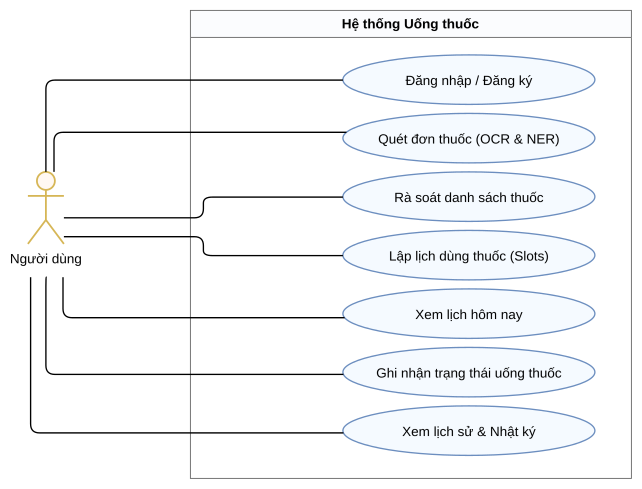
\includegraphics[width=0.96\textwidth]{assets/diagrams/UseCase.pdf}
\caption{Sơ đồ UseCase của hệ thống}
\label{fig:use-case}
\end{figure}

Sơ đồ này chỉ tập trung vào luồng chính của đề tài, từ đăng nhập, quét đơn thuốc, rà soát danh sách thuốc, lập lịch đến theo dõi trong ngày. Việc tách riêng bước rà soát kết quả quét cho thấy hệ thống không dùng kết quả nhận diện như quyết định cuối cùng mà luôn giữ quyền xác nhận ở phía người dùng.

\section{Yêu cầu phi chức năng}

Ngoài chức năng, hệ thống phải đáp ứng các yêu cầu phi chức năng sau:

\begin{itemize}[leftmargin=1.5cm]
    \item \textbf{Tính khả dụng:} luồng chính phải đủ đơn giản để người dùng phổ thông có thể thực hiện mà không cần hiểu cấu trúc dữ liệu bên trong hệ thống.
    \item \textbf{Tính phản hồi:} thời gian xử lý ảnh cần ở mức chấp nhận được để không làm gián đoạn trải nghiệm người dùng.
    \item \textbf{Tính ổn định:} máy chủ và mô-đun AI cần tách biệt để lỗi ở một tầng không phá vỡ hoàn toàn các tầng còn lại.
    \item \textbf{Tính an toàn sử dụng:} người dùng phải có bước rà soát kết quả nhận diện trước khi lưu kế hoạch, tránh phụ thuộc hoàn toàn vào kết quả tự động.
    \item \textbf{Khả năng mở rộng:} kiến trúc cần cho phép mở rộng thêm chức năng trong tương lai như đồng bộ dữ liệu, phân tích đơn sâu hơn hoặc hỗ trợ nhiều đối tượng người dùng hơn.
\end{itemize}

\section{Kiến trúc tổng thể}

Kiến trúc tổng thể của hệ thống gồm ba lớp riêng biệt: ứng dụng di động, máy chủ và mô-đun AI. Ứng dụng di động chịu trách nhiệm tương tác với người dùng. Máy chủ chịu trách nhiệm điều phối nghiệp vụ, xác thực, lưu trữ và cung cấp dữ liệu. Mô-đun AI chuyên xử lý ảnh đơn thuốc và trả về kết quả nhận diện.

\begin{figure}[tbp]
\centering
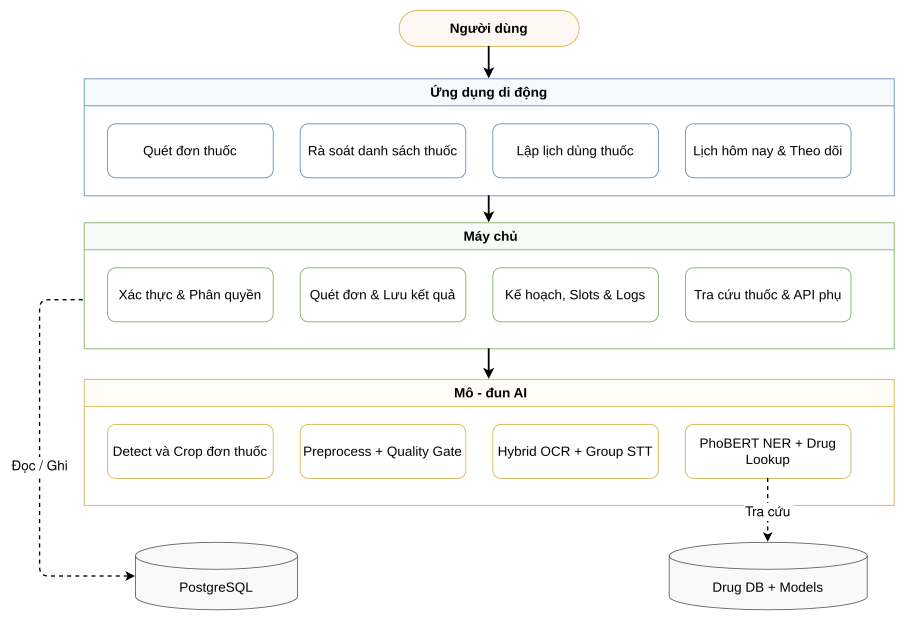
\includegraphics[width=0.94\textwidth]{assets/diagrams/PhanTang.pdf}
\caption{Kiến trúc tổng thể của hệ thống}
\label{fig:overall-architecture}
\end{figure}

Như được thể hiện chi tiết trên sơ đồ, hệ thống được phân chia rõ làm ba nền tảng chính có tính độc lập cao. Ứng dụng di động đóng vai trò là giao diện trực quan, chịu trách nhiệm xử lý các tác vụ phản hồi trên máy khách. Máy chủ Node.js đóng vai trò là xương sống kết nối và điều hướng dữ liệu người dùng vào PostgreSQL. Mô-đun AI (FastAPI) đảm nhiệm vai trò hộp đen giúp thực thi suy luận mô hình mạnh mẽ và trả kết quả độc lập qua API nội bộ.

Việc tách thành ba lớp giúp dự án dễ phát triển hơn ở hai khía cạnh. Thứ nhất, ứng dụng di động và máy chủ có thể thay đổi giao diện và nghiệp vụ mà không phải can thiệp sâu vào phần xử lý AI. Thứ hai, phần xử lý AI có thể được kiểm thử và tối ưu riêng mà không làm ảnh hưởng đến dữ liệu trao đổi của toàn hệ thống.

\section{Thiết kế luồng quét đơn thuốc}

Luồng quét đơn thuốc bắt đầu từ khi người dùng chụp ảnh đơn thuốc trên ứng dụng và kết thúc khi danh sách thuốc được trả về để rà soát. Sơ đồ sau mô tả chuỗi trao đổi dữ liệu giữa các thành phần trong luồng này.

Luồng quét đơn thuốc được thiết kế theo thứ tự sau:

\begin{enumerate}[label=\arabic*.]
    \item Người dùng mở màn hình quét và chụp ảnh đơn thuốc.
    \item Ứng dụng kiểm tra sơ bộ chất lượng ảnh ngay trên thiết bị; ảnh quá mờ hoặc quá chói được thông báo ngay để người dùng chụp lại.
    \item Ảnh được gửi lên máy chủ rồi chuyển tiếp đến mô-đun AI.
    \item Mô-đun AI phát hiện và cắt vùng đơn thuốc, sau đó tiền xử lý ảnh để chuẩn bị cho bước nhận diện.
    \item Ảnh qua bước kiểm tra chất lượng lần hai; nếu quá kém, hệ thống yêu cầu chụp lại thay vì tiếp tục xử lý.
    \item Với ảnh đạt yêu cầu, mô-đun tùy chọn khoanh vùng bảng thuốc trước khi chuyển sang bước OCR.
    \item Kết quả OCR được gom theo số thứ tự dòng thuốc, rồi đưa qua bước trích xuất tên thuốc và đối sánh với cơ sở dữ liệu.
    \item Kết quả được trả về máy chủ, định dạng thành danh sách thuốc và gửi về ứng dụng.
    \item Ứng dụng hiển thị danh sách thuốc để người dùng rà soát trước khi lập lịch.
\end{enumerate}

Hình~\ref{fig:sequence-scan} mô tả sơ đồ tuần tự của luồng quét đơn thuốc, thể hiện chuỗi trao đổi dữ liệu giữa ứng dụng, máy chủ và mô-đun AI.

\begin{figure}[tbp]
\centering
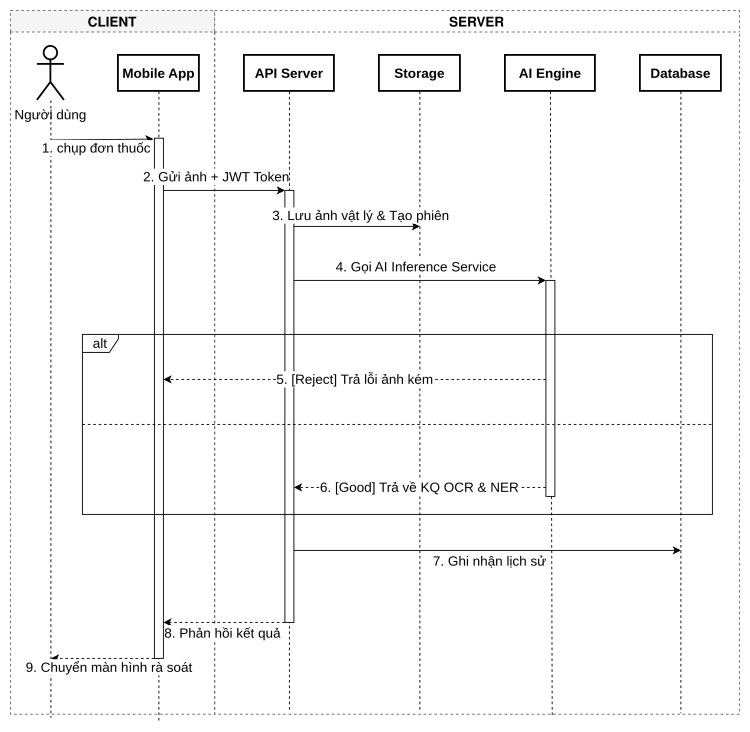
\includegraphics[width=0.85\textwidth,height=0.88\textheight,keepaspectratio]{assets/diagrams/Sequence_ScanFlow.pdf}
\caption{Sơ đồ tuần tự của luồng quét đơn thuốc trong nhánh đánh giá trung tâm}
\label{fig:sequence-scan}
\end{figure}

Hình~\ref{fig:scan-flow} mô tả chi tiết chuỗi xử lý bên trong mô-đun AI, từ bước phát hiện vùng đơn thuốc, kiểm tra chất lượng, nhận diện văn bản đến trích xuất tên thuốc.

\begin{figure}[tbp]
\centering
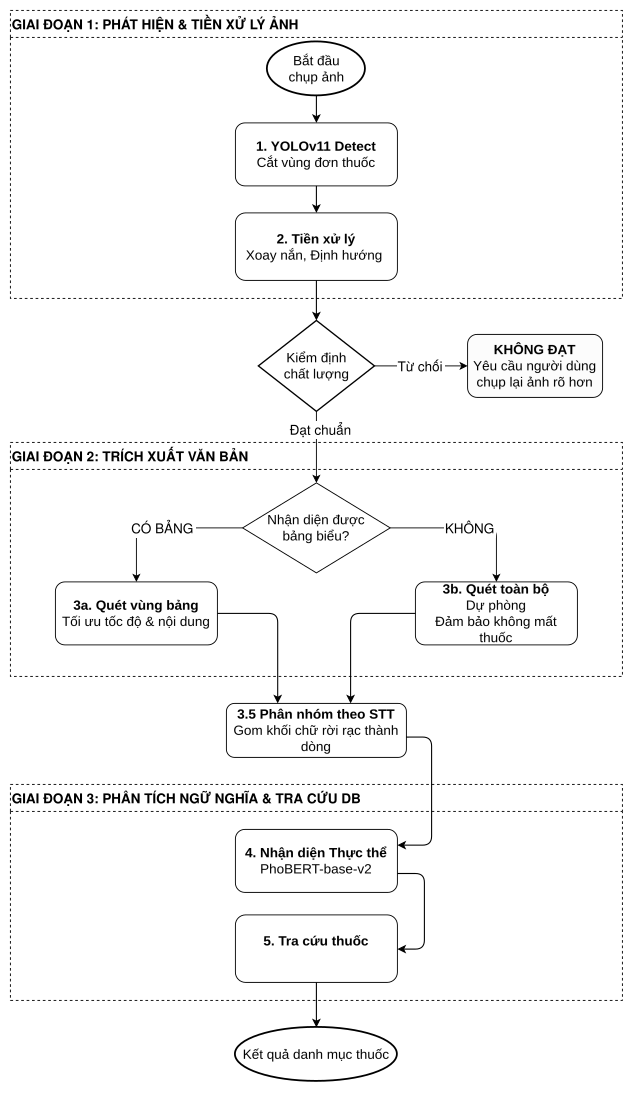
\includegraphics[width=0.82\textwidth,height=0.88\textheight,keepaspectratio]{assets/diagrams/ScanFlow_AI_Pipeline.pdf}
\caption{Sơ đồ luồng xử lý nhận diện đơn thuốc trong Phase A}
\label{fig:scan-flow}
\end{figure}

\section{Thiết kế quy trình xử lý nhận diện đơn thuốc}

Quy trình nhận diện đơn thuốc được chia thành nhiều bước để tăng tính kiểm soát và khả năng gỡ lỗi:

\begin{table}[htbp]
\centering
\caption{Các bước chính trong quy trình nhận diện đơn thuốc}
\label{tab:pipeline-steps}
{\renewcommand{\arraystretch}{1.4}
\begin{tabularx}{\textwidth}{J}
\TableHeader{\textbf{STT} & \textbf{Thành phần} & \textbf{Vai trò}}
\TableRow{1 & Phát hiện và cắt vùng đơn & Phát hiện vùng đơn thuốc và cắt khỏi nền ảnh bằng đường bao lồi để giảm nhiễu nền.}
\TableRow{2 & Tiền xử lý & Chỉnh nghiêng Modulo 90, hiệu chỉnh hướng bằng AI và chuẩn hóa ảnh trước OCR.}
\TableRow{3 & Kiểm tra chất lượng & Đánh giá trạng thái GOOD/WARNING/REJECT để quyết định tiếp tục hay yêu cầu chụp lại.}
\TableRow{4 & Khoanh vùng bảng thuốc (tùy chọn) & Dò vùng bảng thuốc để OCR trong vùng quan tâm, đồng thời giữ OCR dự phòng trên toàn ảnh nếu vùng quan tâm không ổn định.}
\TableRow{5 & Nhận dạng ký tự kết hợp & Dùng PaddleOCR để phát hiện vùng chữ và VietOCR để nhận dạng nội dung tiếng Việt.}
\TableRow{6 & Gom các khối theo số thứ tự dòng thuốc & Gom các khối cùng mục thuốc về chuỗi ổn định hơn trước khi hiểu ngữ nghĩa.}
\TableRow{7 & Trích xuất tên thuốc & Dùng PhoBERT NER để xác định khối văn bản nào có khả năng là tên thuốc.}
\TableRow{8 & Tra cứu thuốc & Đối sánh với cơ sở dữ liệu thuốc Việt Nam để chuẩn hóa và gợi ý tên thuốc.}
\end{tabularx}}
\end{table}

Thiết kế nhiều bước giúp mỗi khâu có thể được kiểm tra độc lập. Nhờ đó, khi kết quả OCR hoặc trích xuất tên thuốc chưa đạt yêu cầu, việc truy vết nguyên nhân được thực hiện rõ ràng hơn theo từng công đoạn, bao gồm chất lượng ảnh đầu vào, cắt vùng đơn, khoanh vùng quan tâm và gom nhóm khối OCR trước bước xử lý ngôn ngữ

\section{Thiết kế dữ liệu kế hoạch dùng thuốc}

Sau khi người dùng xác nhận danh sách thuốc, dữ liệu được chuyển thành một kế hoạch dùng thuốc. Sơ đồ thực thể liên kết mức logic trong Hình~\ref{fig:erd-main} Hai nhóm dữ liệu được ưu tiên là nhóm quét đơn thuốc gồm người dùng, lịch sử quét và bảng phiên quét hỗ trợ cho nhánh nhiều ảnh; cùng với nhóm dữ liệu kế hoạch dùng thuốc gồm kế hoạch, thuốc, khung giờ, bảng nối liều dùng theo khung giờ và nhật ký thực hiện.

\begin{figure}[tbp]
\centering
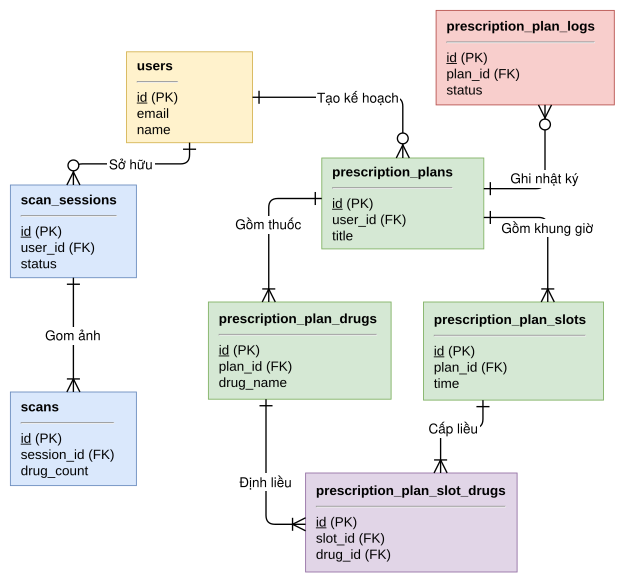
\includegraphics[width=0.95\textwidth,keepaspectratio]{assets/diagrams/ERD_Model.pdf}
\caption{Sơ đồ mô hình thực thể liên kết (ERD) cho luồng dữ liệu chính}
\label{fig:erd-main}
\end{figure}

Một kế hoạch gồm ba phần chính: danh sách thuốc, các khung giờ uống và thông tin liều dùng theo từng khung giờ. Cấu trúc này cho phép một loại thuốc có thể có số viên khác nhau ở các thời điểm khác nhau trong ngày. Ở phía quét đơn, việc tách riêng \path{scan_sessions} và \path{scans} giúp hệ thống lưu lại cả lịch sử quét lẫn trạng thái hội tụ của một phiên quét mà không trộn lẫn với dữ liệu kế hoạch dùng thuốc. Tuy nhiên, \path{scan_sessions} chỉ đóng vai trò bảng hỗ trợ cho nhánh quét nhiều ảnh, không phải là tâm của sơ đồ tuần tự đã chọn làm luồng minh họa chính.

Ở máy chủ, dữ liệu được tách thành nhiều bảng để dễ quản lý: bảng kế hoạch tổng quát (\path{prescription_plans}), bảng thuốc trong kế hoạch (\path{prescription_plan_drugs}), bảng khung giờ (\path{prescription_plan_slots}) và bảng nối n-n quy định số viên theo từng khung giờ (\path{prescription_plan_slot_drugs}). Riêng bảng nhật ký \path{prescription_plan_logs} bám theo kế hoạch để lưu trạng thái thực hiện theo từng lần uống, thay vì liên kết trực tiếp sang bảng nối liều dùng. Cách tách này đủ để biểu diễn luồng chính mà không phải đưa thêm các bảng về tương tác thuốc, pill verification hoặc pill reference vào ERD trung tâm.

Để người đọc dễ đối chiếu sơ đồ với schema thật, Bảng~\ref{tab:erd-entities} tóm tắt vai trò của từng thực thể chính.

\begin{table}[htbp]
\centering
\caption{Vai trò của các thực thể chính trong ERD}
\label{tab:erd-entities}
{\renewcommand{\arraystretch}{1.35}
\begin{tabularx}{\textwidth}{J}
\TableHeader{\textbf{STT} & \textbf{Thực thể} & \textbf{Vai trò trong luồng chính}}
\TableRow{1 & \path{users} & Lưu thông tin tài khoản và là thực thể gốc để gắn lịch sử quét cũng như kế hoạch dùng thuốc.}
\TableRow{2 & \path{scan_sessions} & Gom nhiều ảnh quét trong nhánh mở rộng quét nhiều lần; được giữ lại trong ERD để phản ánh schema thật nhưng không phải tâm của luồng minh họa chính.}
\TableRow{3 & \path{scans} & Lưu từng lần quét, kết quả nhận diện, trạng thái chất lượng ảnh và số lượng thuốc trích xuất được.}
\TableRow{4 & \path{prescription_plans} & Lưu thông tin tổng quát của một kế hoạch dùng thuốc như tiêu đề, ngày bắt đầu, ngày kết thúc và trạng thái hoạt động.}
\TableRow{5 & \path{prescription_plan_drugs} & Lưu danh sách thuốc nằm trong một kế hoạch và giữ thứ tự hiển thị của từng thuốc.}
\TableRow{6 & \path{prescription_plan_slots} & Lưu các khung giờ uống trong ngày của một kế hoạch.}
\TableRow{7 & \path{prescription_plan_slot_drugs} & Là bảng nối giữa thuốc và khung giờ, đồng thời lưu số viên phải uống của từng thuốc tại từng khung giờ.}
\TableRow{8 & \path{prescription_plan_logs} & Lưu nhật ký thực hiện theo từng lần uống để phục vụ màn hình hôm nay và lịch sử theo dõi.}
\end{tabularx}}
\end{table}

\subsection{Mô tả các thực thể chính trong ERD}

Để phần dữ liệu có cách trình bày gần với mẫu báo cáo tham khảo hơn, mỗi thực thể chính trong ERD được mô tả lại bằng một bảng thuộc tính riêng. Các bảng dưới đây chỉ tập trung vào các thuộc tính chính đang được thể hiện trực tiếp trên sơ đồ logic, thay vì liệt kê toàn bộ schema kỹ thuật của hệ thống.

\subsubsection{Bảng users}

Đây là thực thể gốc dùng để xác định chủ sở hữu của dữ liệu quét đơn thuốc và kế hoạch dùng thuốc.

\begin{table}[H]
\centering
\caption{Các thuộc tính chính của thực thể users}
\label{tab:entity-users}
{\footnotesize\renewcommand{\arraystretch}{1.25}
\begin{tabularx}{\textwidth}{Q}
\TableHeader{\textbf{STT} & \textbf{Tên} & \textbf{Kiểu dữ liệu} & \textbf{Mô tả} & \textbf{Khóa}}
\TableRow{1 & \path{id} & UUID & Mã định danh duy nhất của người dùng. & Khóa chính}
\TableRow{2 & \path{email} & VARCHAR(255) & Địa chỉ thư điện tử dùng để đăng nhập. & }
\TableRow{3 & \path{name} & VARCHAR(100) & Tên hiển thị của người dùng trong ứng dụng. & }
\TableRow{4 & \path{created_at} & TIMESTAMPTZ & Thời điểm tạo tài khoản. & }
\end{tabularx}}
\end{table}

\subsubsection{Bảng scan\_sessions}

Thực thể này hỗ trợ nhánh quét nhiều ảnh và gom các lần quét lại thành một phiên chung.

\begin{table}[H]
\centering
\caption{Các thuộc tính chính của thực thể scan\_sessions}
\label{tab:entity-scan-sessions}
{\footnotesize\renewcommand{\arraystretch}{1.25}
\begin{tabularx}{\textwidth}{Q}
\TableHeader{\textbf{STT} & \textbf{Tên} & \textbf{Kiểu dữ liệu} & \textbf{Mô tả} & \textbf{Khóa}}
\TableRow{1 & \path{id} & UUID & Mã định danh của một phiên quét nhiều ảnh. & Khóa chính}
\TableRow{2 & \path{user_id} & UUID & Người dùng sở hữu phiên quét. & Khóa ngoại}
\TableRow{3 & \path{status} & VARCHAR(20) & Trạng thái của phiên, ví dụ đang mở hoặc đã dừng. & }
\TableRow{4 & \path{converged} & BOOLEAN & Cờ đánh dấu kết quả phiên đã hội tụ hay chưa. & }
\TableRow{5 & \path{merged_result} & JSONB & Danh sách thuốc hợp nhất sau nhiều lần quét trong cùng phiên. & }
\end{tabularx}}
\end{table}

\subsubsection{Bảng scans}

Đây là bảng lưu lịch sử từng lần quét đơn thuốc của người dùng trong hệ thống.

\begin{table}[H]
\centering
\caption{Các thuộc tính chính của thực thể scans}
\label{tab:entity-scans}
{\footnotesize\renewcommand{\arraystretch}{1.25}
\begin{tabularx}{\textwidth}{Q}
\TableHeader{\textbf{STT} & \textbf{Tên} & \textbf{Kiểu dữ liệu} & \textbf{Mô tả} & \textbf{Khóa}}
\TableRow{1 & \path{id} & UUID & Mã định danh của một lần quét cụ thể. & Khóa chính}
\TableRow{2 & \path{user_id} & UUID & Người dùng thực hiện lần quét đó. & Khóa ngoại}
\TableRow{3 & \path{session_id} & UUID & Phiên quét liên quan nếu người dùng dùng nhánh quét nhiều ảnh. & Khóa ngoại}
\TableRow{4 & \path{quality_state} & VARCHAR(20) & Trạng thái chất lượng ảnh sau bước đánh giá. & }
\TableRow{5 & \path{drug_count} & INTEGER & Số lượng thuốc mà hệ thống trích xuất được từ lần quét. & }
\end{tabularx}}
\end{table}

\subsubsection{Bảng prescription\_plans}

Đây là bảng trung tâm của nhóm dữ liệu kế hoạch dùng thuốc, lưu thông tin khái quát của một kế hoạch.

\begin{table}[H]
\centering
\caption{Các thuộc tính chính của thực thể prescription\_plans}
\label{tab:entity-prescription-plans}
{\footnotesize\renewcommand{\arraystretch}{1.25}
\begin{tabularx}{\textwidth}{Q}
\TableHeader{\textbf{STT} & \textbf{Tên} & \textbf{Kiểu dữ liệu} & \textbf{Mô tả} & \textbf{Khóa}}
\TableRow{1 & \path{id} & UUID & Mã định danh của kế hoạch dùng thuốc. & Khóa chính}
\TableRow{2 & \path{user_id} & UUID & Người dùng sở hữu kế hoạch. & Khóa ngoại}
\TableRow{3 & \path{title} & VARCHAR(255) & Tiêu đề hoặc tên gợi nhớ cho kế hoạch. & }
\TableRow{4 & \path{start_date} & DATE & Ngày bắt đầu áp dụng kế hoạch. & }
\TableRow{5 & \path{end_date} & DATE & Ngày kết thúc kế hoạch nếu đã xác định. & }
\TableRow{6 & \path{is_active} & BOOLEAN & Trạng thái cho biết kế hoạch còn hiệu lực hay không. & }
\end{tabularx}}
\end{table}

\subsubsection{Bảng prescription\_plan\_drugs}

Thực thể này lưu danh sách thuốc thuộc về một kế hoạch cụ thể.

\begin{table}[H]
\centering
\caption{Các thuộc tính chính của thực thể prescription\_plan\_drugs}
\label{tab:entity-prescription-plan-drugs}
{\footnotesize\renewcommand{\arraystretch}{1.25}
\begin{tabularx}{\textwidth}{Q}
\TableHeader{\textbf{STT} & \textbf{Tên} & \textbf{Kiểu dữ liệu} & \textbf{Mô tả} & \textbf{Khóa}}
\TableRow{1 & \path{id} & UUID & Mã định danh của một thuốc trong kế hoạch. & Khóa chính}
\TableRow{2 & \path{plan_id} & UUID & Kế hoạch chứa thuốc đó. & Khóa ngoại}
\TableRow{3 & \path{drug_name} & VARCHAR(255) & Tên thuốc hiển thị cho người dùng. & }
\TableRow{4 & \path{dosage} & VARCHAR(100) & Hàm lượng hoặc quy cách ngắn của thuốc. & }
\TableRow{5 & \path{sort_order} & INTEGER & Thứ tự hiển thị của thuốc trong danh sách kế hoạch. & }
\end{tabularx}}
\end{table}

\subsubsection{Bảng prescription\_plan\_slots}

Thực thể này mô tả các khung giờ uống thuốc trong ngày của một kế hoạch.

\begin{table}[H]
\centering
\caption{Các thuộc tính chính của thực thể prescription\_plan\_slots}
\label{tab:entity-prescription-plan-slots}
{\footnotesize\renewcommand{\arraystretch}{1.25}
\begin{tabularx}{\textwidth}{Q}
\TableHeader{\textbf{STT} & \textbf{Tên} & \textbf{Kiểu dữ liệu} & \textbf{Mô tả} & \textbf{Khóa}}
\TableRow{1 & \path{id} & UUID & Mã định danh của một khung giờ uống thuốc. & Khóa chính}
\TableRow{2 & \path{plan_id} & UUID & Kế hoạch sở hữu khung giờ này. & Khóa ngoại}
\TableRow{3 & \path{time} & VARCHAR(5) & Thời điểm uống theo định dạng giờ và phút. & }
\TableRow{4 & \path{sort_order} & INTEGER & Thứ tự sắp xếp của khung giờ trên giao diện. & }
\end{tabularx}}
\end{table}

\subsubsection{Bảng prescription\_plan\_slot\_drugs}

Đây là bảng nối giữa thuốc và khung giờ, cho phép khai báo số viên khác nhau ở từng thời điểm trong ngày.

\begin{table}[H]
\centering
\caption{Các thuộc tính chính của thực thể prescription\_plan\_slot\_drugs}
\label{tab:entity-prescription-plan-slot-drugs}
{\footnotesize\renewcommand{\arraystretch}{1.25}
\begin{tabularx}{\textwidth}{Q}
\TableHeader{\textbf{STT} & \textbf{Tên} & \textbf{Kiểu dữ liệu} & \textbf{Mô tả} & \textbf{Khóa}}
\TableRow{1 & \path{id} & UUID & Mã định danh của liên kết giữa khung giờ và thuốc. & Khóa chính}
\TableRow{2 & \path{slot_id} & UUID & Khung giờ được áp dụng liều dùng. & Khóa ngoại}
\TableRow{3 & \path{drug_id} & UUID & Thuốc được gán vào khung giờ tương ứng. & Khóa ngoại}
\TableRow{4 & \path{pills} & INTEGER & Số viên phải uống của thuốc tại khung giờ đó. & }
\end{tabularx}}
\end{table}

\subsubsection{Bảng prescription\_plan\_logs}

Thực thể này lưu lại trạng thái thực hiện của từng lần uống để phục vụ màn hình theo dõi hôm nay và lịch sử.

\begin{table}[H]
\centering
\caption{Các thuộc tính chính của thực thể prescription\_plan\_logs}
\label{tab:entity-prescription-plan-logs}
{\footnotesize\renewcommand{\arraystretch}{1.25}
\begin{tabularx}{\textwidth}{Q}
\TableHeader{\textbf{STT} & \textbf{Tên} & \textbf{Kiểu dữ liệu} & \textbf{Mô tả} & \textbf{Khóa}}
\TableRow{1 & \path{id} & UUID & Mã định danh của một bản ghi nhật ký dùng thuốc. & Khóa chính}
\TableRow{2 & \path{plan_id} & UUID & Kế hoạch tạo ra lần uống cần theo dõi. & Khóa ngoại}
\TableRow{3 & \path{occurrence_id} & VARCHAR(120) & Mã duy nhất đại diện cho một lần uống cụ thể. & }
\TableRow{4 & \path{slot_time} & VARCHAR(5) & Khung giờ gốc của lần uống được ghi nhận. & }
\TableRow{5 & \path{status} & VARCHAR(20) & Trạng thái thực hiện như \texttt{taken}, \texttt{missed}, \texttt{skipped} hoặc \texttt{pending}. & }
\end{tabularx}}
\end{table}

Để mô phỏng hành vi thiết lập lịch từ phía người dùng trên giao diện, Sơ đồ hoạt động ở Hình~\ref{fig:activity-create-plan} mô tả rõ các bước mà người dùng có thể thực hiện khi nhận được kết quả quét từ hệ thống.

\begin{figure}[tbp]
\centering
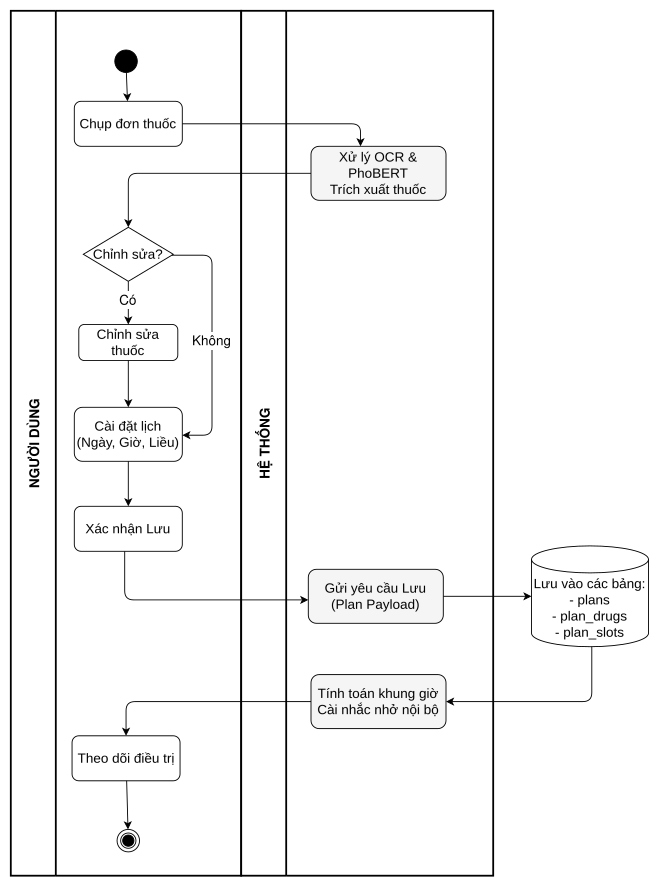
\includegraphics[width=0.82\textwidth,height=0.88\textheight,keepaspectratio]{assets/diagrams/Activity_CreatePlan.pdf}
\caption{Sơ đồ hoạt động cho luồng tạo kế hoạch dùng thuốc}
\label{fig:activity-create-plan}
\end{figure}

Sơ đồ đã làm nổi bật hai nhánh chính là chỉnh sửa danh sách thuốc khi cần và khai báo liều lượng chi tiết thông qua các khung giờ. Những thay đổi này được thiết lập ở bộ nhớ tạm của thiết bị và chỉ được gửi về máy chủ khi người dùng xác nhận lưu kế hoạch.

\section{Thiết kế nhật ký dùng thuốc và theo dõi trong ngày}

Để hỗ trợ theo dõi việc uống thuốc, hệ thống tạo ra mã định danh cho từng lần uống. Mỗi mã định danh tương ứng với một kế hoạch, một ngày và một khung giờ cụ thể. Khi người dùng xác nhận đã uống hoặc bỏ qua, máy chủ lưu trạng thái vào bảng nhật ký. Thiết kế này giúp tránh việc ghi trùng khi người dùng thao tác lại hoặc khi ứng dụng cần đồng bộ lại trạng thái từ thiết bị.

\section{Các quyết định thiết kế quan trọng}

\subsection{Ưu tiên luồng chính thay vì mở rộng quá sớm}

Một quyết định quan trọng của đề tài là ưu tiên hoàn thiện luồng có giá trị thực tế cao nhất gồm quét đơn thuốc, rà soát kết quả và lập lịch dùng thuốc. Thay vì cố gắng mở rộng ngay sang nhiều chức năng phức tạp khác, đề tài tập trung làm tốt phần đầu cuối đang phục vụ trực tiếp cho người dùng.

\subsection{Không để đối sánh tên thuốc ghi đè hoàn toàn văn bản nhận dạng}

Trong thực tế, đối sánh gần đúng có thể giúp chuẩn hóa dữ liệu nhưng cũng có thể đưa ra ứng viên sai. Vì vậy, hệ thống giữ văn bản nhận dạng được như nguồn hiển thị chính và dùng kết quả đối sánh như thông tin bổ sung hỗ trợ. Điều này làm tăng tính minh bạch cho người dùng khi rà soát lại kết quả quét.

\subsection{Không tích hợp ngay chức năng xác minh viên thuốc qua hình ảnh}

Đề tài đã khảo sát hướng xác minh viên thuốc bằng ảnh đầu vào của người dùng, kết hợp đối sánh theo tên thuốc, màu sắc, hình dạng và dạng bào chế. Tuy nhiên, hướng này mới dừng ở mức thử nghiệm trong dự án và chưa được đưa vào phạm vi đánh giá trung tâm vì độ an toàn chưa đủ cao. Phần phân tích chi tiết được trình bày ở Chương 5.

\chapter{CÀI ĐẶT HỆ THỐNG}

\section{Môi trường phát triển}

Hệ thống được phát triển trong môi trường gồm Python 3.12 cho mô-đun AI, Node.js 20 cho máy chủ, PostgreSQL 16 cho lưu trữ và Flutter cho ứng dụng di động. Về mặt phần cứng, quá trình phát triển và thử nghiệm trí tuệ nhân tạo được tối ưu cho GPU RTX 3050 4GB, đồng thời vẫn duy trì khả năng chuyển sang chế độ dự phòng bằng CPU trong một số tình huống.

\begin{table}[htbp]
\centering
\caption{Môi trường phát triển chính của hệ thống}
\label{tab:environment}
{\renewcommand{\arraystretch}{1.4}
\begin{tabularx}{\textwidth}{J}
\TableHeader{\textbf{STT} & \textbf{Thành phần} & \textbf{Mô tả}}
\TableRow{1 & Ngôn ngữ mô-đun AI & Python 3.12}
\TableRow{2 & Ngôn ngữ máy chủ & Node.js 20}
\TableRow{3 & Khung chương trình máy chủ & FastAPI, Express 4}
\TableRow{4 & Ứng dụng di động & Flutter, Dart SDK 3.10.x}
\TableRow{5 & Hệ quản trị cơ sở dữ liệu & PostgreSQL 16}
\TableRow{6 & Mô hình nhận dạng và ngôn ngữ & PaddleOCR, VietOCR, PhoBERT}
\TableRow{7 & Thiết bị tăng tốc & GPU RTX 3050 4GB hoặc CPU dự phòng}
\end{tabularx}}
\end{table}

\section{Cài đặt mô-đun quét đơn thuốc}

Mô-đun quét đơn thuốc được triển khai trong mô-đun AI viết bằng Python. Thành phần điều phối có nhiệm vụ nối các bước xử lý thành một chuỗi thống nhất. Ở mức tách lớp, các bước phát hiện/cắt vùng, tiền xử lý, kiểm tra chất lượng, OCR, gom các khối theo số thứ tự dòng thuốc, trích xuất tên thuốc và tra cứu thuốc được đặt ở các thư mục riêng để dễ gỡ lỗi và kiểm thử.

Trong quá trình triển khai, bước phát hiện đơn thuốc bằng YOLO được dùng để tách phần tờ đơn ra khỏi nền ảnh theo đường bao lồi. Sau đó ảnh được nắn thẳng góc theo Modulo 90 và hiệu chỉnh hướng bằng mô hình AI để bộ OCR hoạt động ổn định hơn. Sau kiểm tra chất lượng, hệ thống có thể dò khoanh vùng bảng thuốc theo hướng tùy chọn trước khi đưa qua OCR. Kết quả nhận dạng tiếp tục được gom theo số thứ tự dòng thuốc, rồi mới đi qua PhoBERT để lọc ra các đoạn có khả năng là tên thuốc trước khi đối sánh với cơ sở dữ liệu thuốc Việt Nam.

Để trực quan hóa kết quả của giai đoạn đầu tiên này, Hình~\ref{fig:preprocessed} trình bày trạng thái của ảnh đơn thuốc sau khi đã được mô hình YOLO cắt lọc bỏ lớp nền nhiễu, deskew và hiệu chỉnh hướng để văn bản nằm ổn định hơn cho bước OCR.

\begin{figure}[tbp]
\centering
\includegraphics[width=0.7\textwidth]{assets/real_data/cropDonThuoc.pdf}
\caption{Kết quả ảnh đơn thuốc sau thao tác cắt nền và nắn chỉnh độ nghiêng}
\label{fig:preprocessed}
\end{figure}

Nhờ tối ưu hóa bước chỉnh hướng, nền ảnh sạch gọn và văn bản duy trì phương ngang chuẩn xác hơn. Đây là thao tác tạo tiền đề đặc biệt có ý nghĩa đối với độ tin cậy của thuật toán phân rã chuỗi nhận dạng ký tự quang học ở ngay khâu kế tiếp.

\section{Cài đặt máy chủ}

Máy chủ được tổ chức theo mô hình tách riêng phần định tuyến, phần xử lý nghiệp vụ và phần tiện ích hỗ trợ. Các phần định tuyến kiểm tra dữ liệu đầu vào bằng Zod, sau đó chuyển sang phần xử lý nghiệp vụ tương ứng. Dữ liệu được trả về theo cấu trúc JSON thống nhất để ứng dụng di động có thể sử dụng trực tiếp.

Trong luồng quét đơn thuốc, máy chủ nhận ảnh từ ứng dụng di động, chuyển tiếp sang FastAPI dưới dạng tệp tải lên, sau đó chuẩn hóa kết quả nhận diện về một cấu trúc ổn định hơn cho ứng dụng di động. Máy chủ cũng lưu lịch sử quét, trạng thái chất lượng ảnh và các thông tin tổng hợp khác phục vụ cho API history cũng như nhu cầu theo dõi hệ thống ở phía máy chủ.

Các nhóm API ở thời điểm hiện tại có thể chia thành hai lớp: lớp phục vụ trực tiếp cho luồng scan -> review -> schedule -> track của đề tài, và lớp phụ trợ hoặc thử nghiệm đã tồn tại trong dự án nhưng không phải trọng tâm đánh giá. Bảng~\ref{tab:api-groups} tóm tắt các nhóm này.

\begin{table}[htbp]
\centering
\caption{Các nhóm API chính của hệ thống ở thời điểm hiện tại}
\label{tab:api-groups}
{\renewcommand{\arraystretch}{1.4}
\begin{tabularx}{\textwidth}{K}
\TableHeader{\textbf{STT} & \textbf{Nhóm} & \textbf{Ví dụ đường dẫn} & \textbf{Vai trò}}
\TableRow{1 & Health & \path{/api/health} & Kiểm tra trạng thái sẵn sàng của backend.}
\TableRow{2 & Xác thực & \texttt{/api/auth/...} & Đăng ký, đăng nhập, refresh token và quản lý người dùng.}
\TableRow{3 & Quét đơn core & \path{/api/scan}, \path{/api/scan/history/...} & Nhận ảnh đơn thuốc, lưu lịch sử quét và trả kết quả cho màn hình rà soát.}
\TableRow{4 & Scan session mở rộng & \path{/api/scan/session/...} & Hỗ trợ nhánh quét thích nghi nhiều ảnh; tồn tại trong dự án nhưng không phải luồng minh họa chính của đề tài.}
\TableRow{5 & Kế hoạch và nhật ký & \path{/api/plans/...} & Quản lý kế hoạch, liều dùng trong ngày, các endpoint today summary và trạng thái \texttt{taken/missed/skipped}.}
\TableRow{6 & Tra cứu thuốc & \path{/api/drugs/...}, \path{/api/drug-interactions/...} & Tìm kiếm thuốc, tra cứu hoạt chất và kiểm tra tương tác như các chức năng phụ trợ.}
\TableRow{7 & Pill verification & \path{/api/pill-verifications/...} & Thành phần thử nghiệm cho hướng xác minh viên thuốc; chưa thuộc luồng đánh giá trung tâm.}
\TableRow{8 & Pill reference & \path{/api/pill-references/...} & Quản lý ảnh tham chiếu viên thuốc cho hướng thử nghiệm tương ứng.}
\end{tabularx}}
\end{table}

\section{Cài đặt ứng dụng di động}

Ứng dụng di động được phát triển bằng Flutter, sử dụng Riverpod cho quản lý trạng thái và Go Router cho điều hướng. Luồng tạo kế hoạch được chia thành nhiều màn hình nhỏ để người dùng không phải xử lý quá nhiều thông tin trong cùng một màn hình.

\subsection{Giao diện màn hình quét đơn}

Ở màn hình quét đơn (Hình~\ref{fig:scan-camera}), ứng dụng mở camera trực tiếp và người dùng chủ động bấm chụp ảnh. Sau khi chụp, ảnh được kiểm tra chất lượng cục bộ để quyết định chụp lại ngay, tiếp tục với cảnh báo, hoặc gửi ảnh lên máy chủ. Tùy chọn nhập tay hoặc dùng lại kế hoạch cũ không nằm trong màn hình camera mà được đặt ở màn hình chọn cách tạo kế hoạch ban đầu.

\begin{figure}[H]
\centering
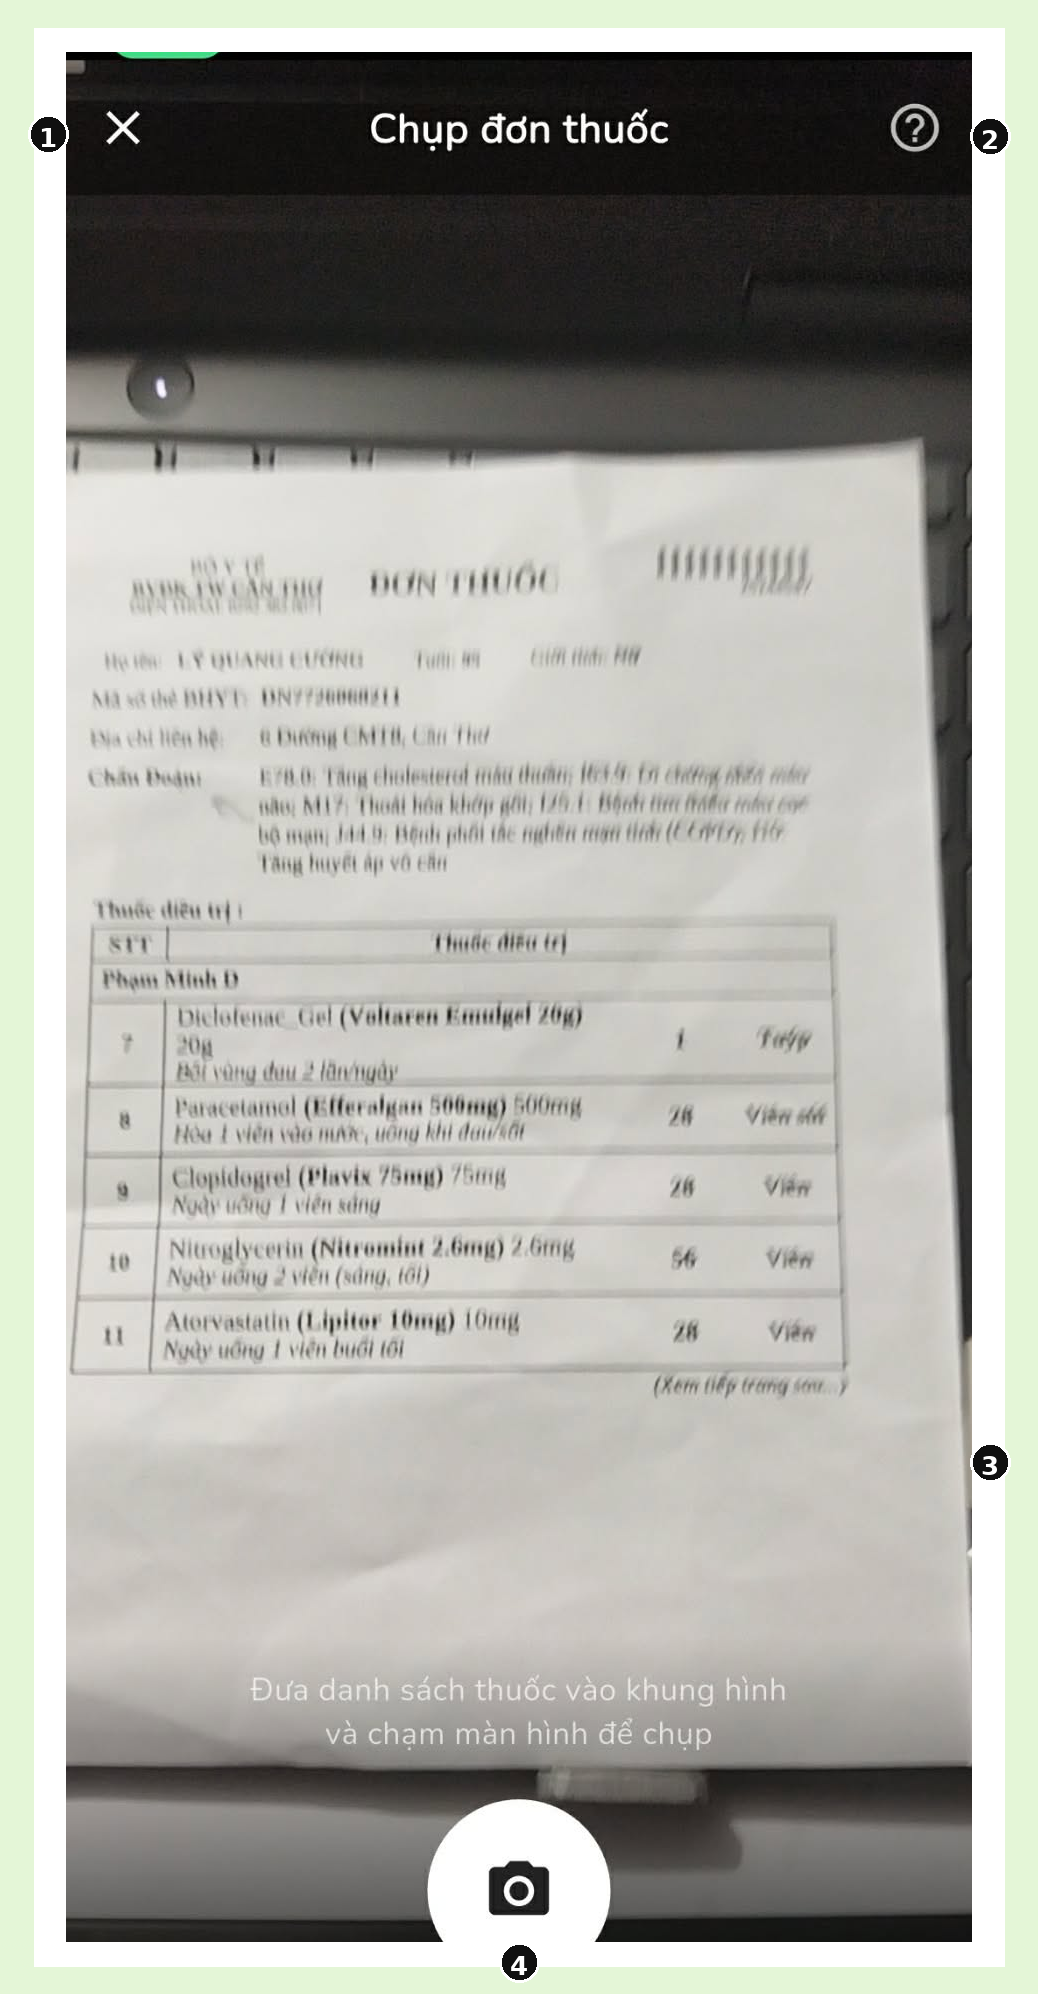
\includegraphics[width=0.52\textwidth]{assets/app/scan_camera_annotated.png}
\caption{Màn hình quét đơn thuốc trên ứng dụng di động}
\label{fig:scan-camera}
\end{figure}

Các thành phần chính của màn hình quét đơn được trình bày trong Bảng~\ref{tab:scan-camera-components}.

\begin{table}[H]
\centering
\caption{Các thành phần của màn hình quét đơn}
\label{tab:scan-camera-components}
{\renewcommand{\arraystretch}{1.35}
\begin{tabularx}{\textwidth}{J}
\TableHeader{\textbf{STT} & \textbf{Thành phần} & \textbf{Mô tả}}
\TableRow{1 & Nút quay lại & Đưa người dùng trở về bước chọn cách tạo kế hoạch nếu chưa muốn tiếp tục quét.}
\TableRow{2 & Nút trợ giúp & Mở phần hướng dẫn thao tác chụp ảnh đơn thuốc đúng khung nhìn.}
\TableRow{3 & Vùng căn đơn thuốc & Khu vực preview để người dùng đặt bảng thuốc vào giữa khung trước khi chụp.}
\TableRow{4 & Nút chụp ảnh & Thực hiện thao tác chụp và chuyển ảnh sang bước kiểm tra chất lượng cục bộ.}
\end{tabularx}}
\end{table}

\subsection{Giao diện rà soát kết quả quét}

Sau khi nhận kết quả từ máy chủ, ứng dụng điều hướng sang màn hình rà soát danh sách thuốc (Hình~\ref{fig:scan-review}). Tại đây người dùng có thể chỉnh sửa tên thuốc, thêm hoặc xóa thuốc trước khi sang bước lập lịch. Thiết kế này đảm bảo người dùng luôn có quyền kiểm soát và xác nhận danh sách cuối cùng, thay vì phụ thuộc hoàn toàn vào kết quả nhận diện tự động.

\begin{figure}[H]
\centering
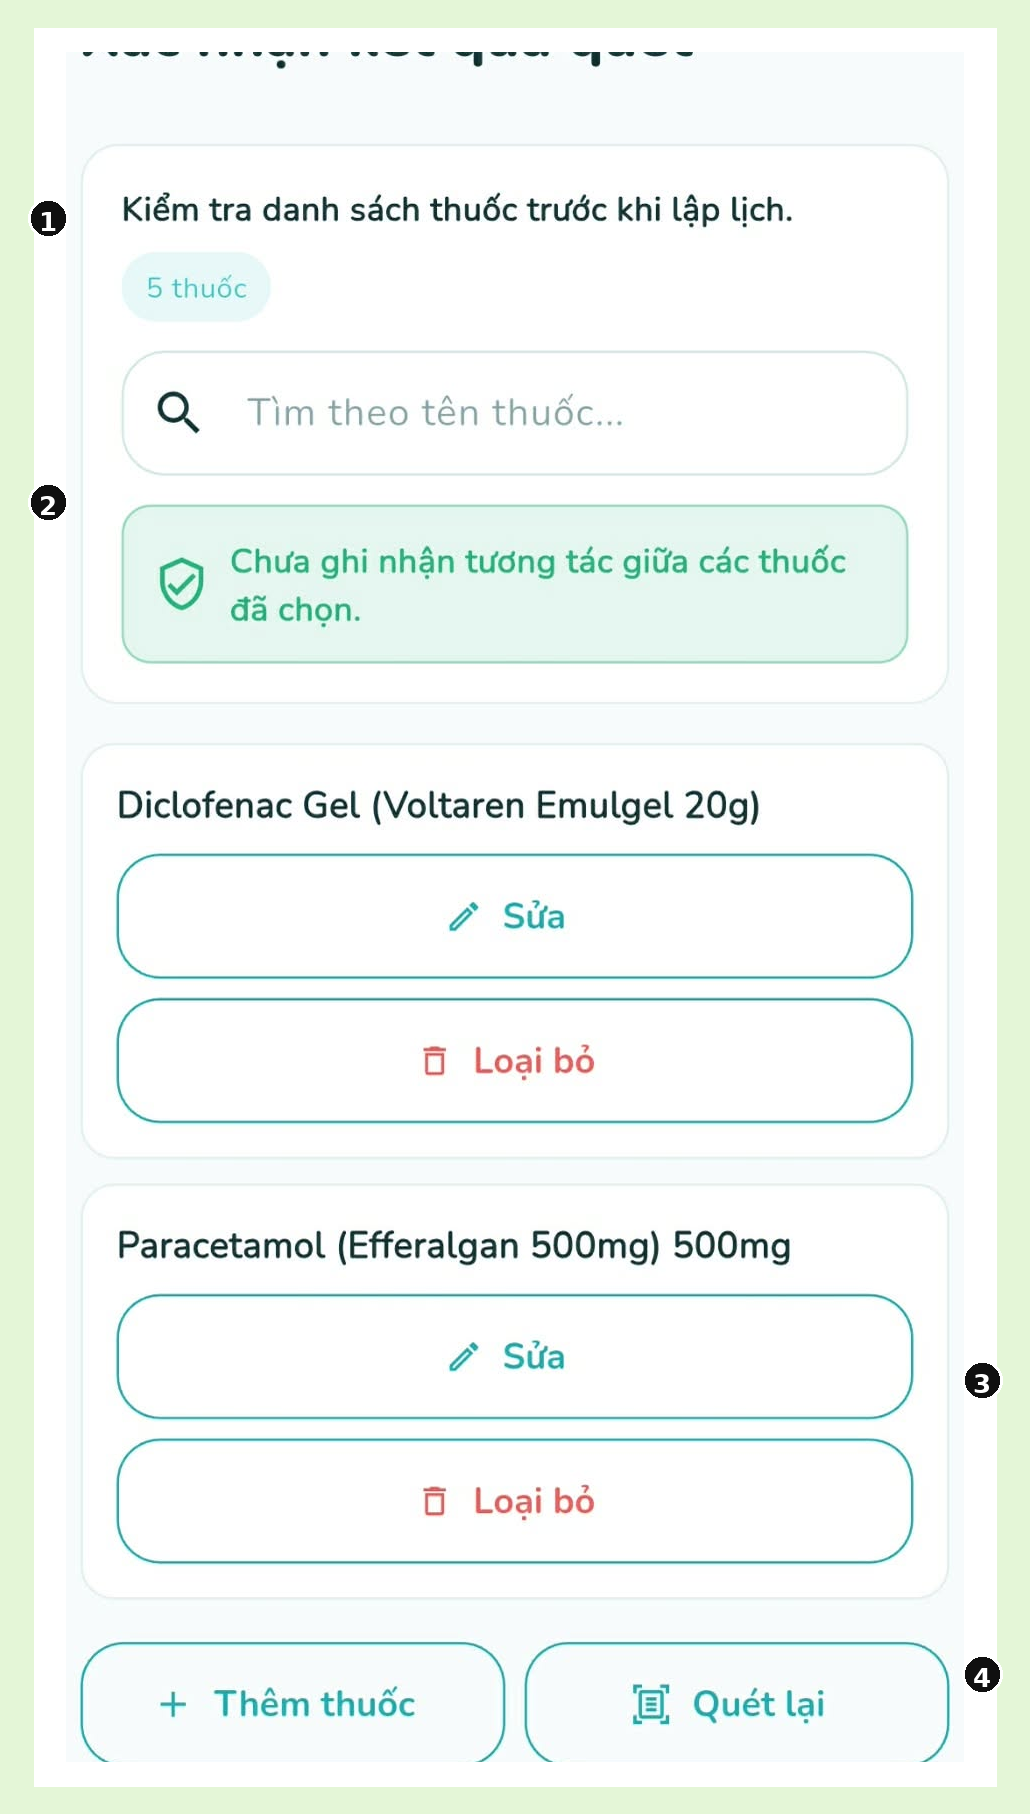
\includegraphics[width=0.52\textwidth]{assets/app/scan_review_annotated.png}
\caption{Màn hình rà soát danh sách thuốc sau khi quét (có thể chỉnh sửa, thêm hoặc xóa từng mục)}
\label{fig:scan-review}
\end{figure}

Các thành phần chính của màn hình rà soát được trình bày trong Bảng~\ref{tab:scan-review-components}.

\begin{table}[H]
\centering
\caption{Các thành phần của màn hình rà soát kết quả quét}
\label{tab:scan-review-components}
{\renewcommand{\arraystretch}{1.35}
\begin{tabularx}{\textwidth}{J}
\TableHeader{\textbf{STT} & \textbf{Thành phần} & \textbf{Mô tả}}
\TableRow{1 & Tiêu đề và bộ đếm thuốc & Cho biết người dùng đang ở bước rà soát và cho biết số mục thuốc đã được nhận diện.}
\TableRow{2 & Khối thông báo an toàn & Hiển thị trạng thái kiểm tra tương tác hoặc cảnh báo nhanh trước khi lập lịch.}
\TableRow{3 & Danh sách thuốc và thao tác chỉnh sửa & Cho phép sửa tên, loại bỏ từng thuốc hoặc kiểm tra lại nội dung trước khi chốt.}
\TableRow{4 & Nhóm thao tác cuối bước & Bao gồm các nút thêm thuốc, quét lại và tiếp tục sang bước lập lịch.}
\end{tabularx}}
\end{table}

\subsection{Giao diện thiết lập lịch dùng thuốc}

Màn hình lập lịch (Hình~\ref{fig:set-schedule}) cho phép người dùng chọn ngày bắt đầu, số ngày dùng, các khung giờ uống và số viên tương ứng cho từng khung giờ. Dữ liệu được xây dựng thành bản nháp kế hoạch rồi gửi lên máy chủ. Sau khi tạo thành công, ứng dụng thiết lập các thông báo nhắc uống cục bộ để nhắc uống thuốc.

\begin{figure}[H]
\centering
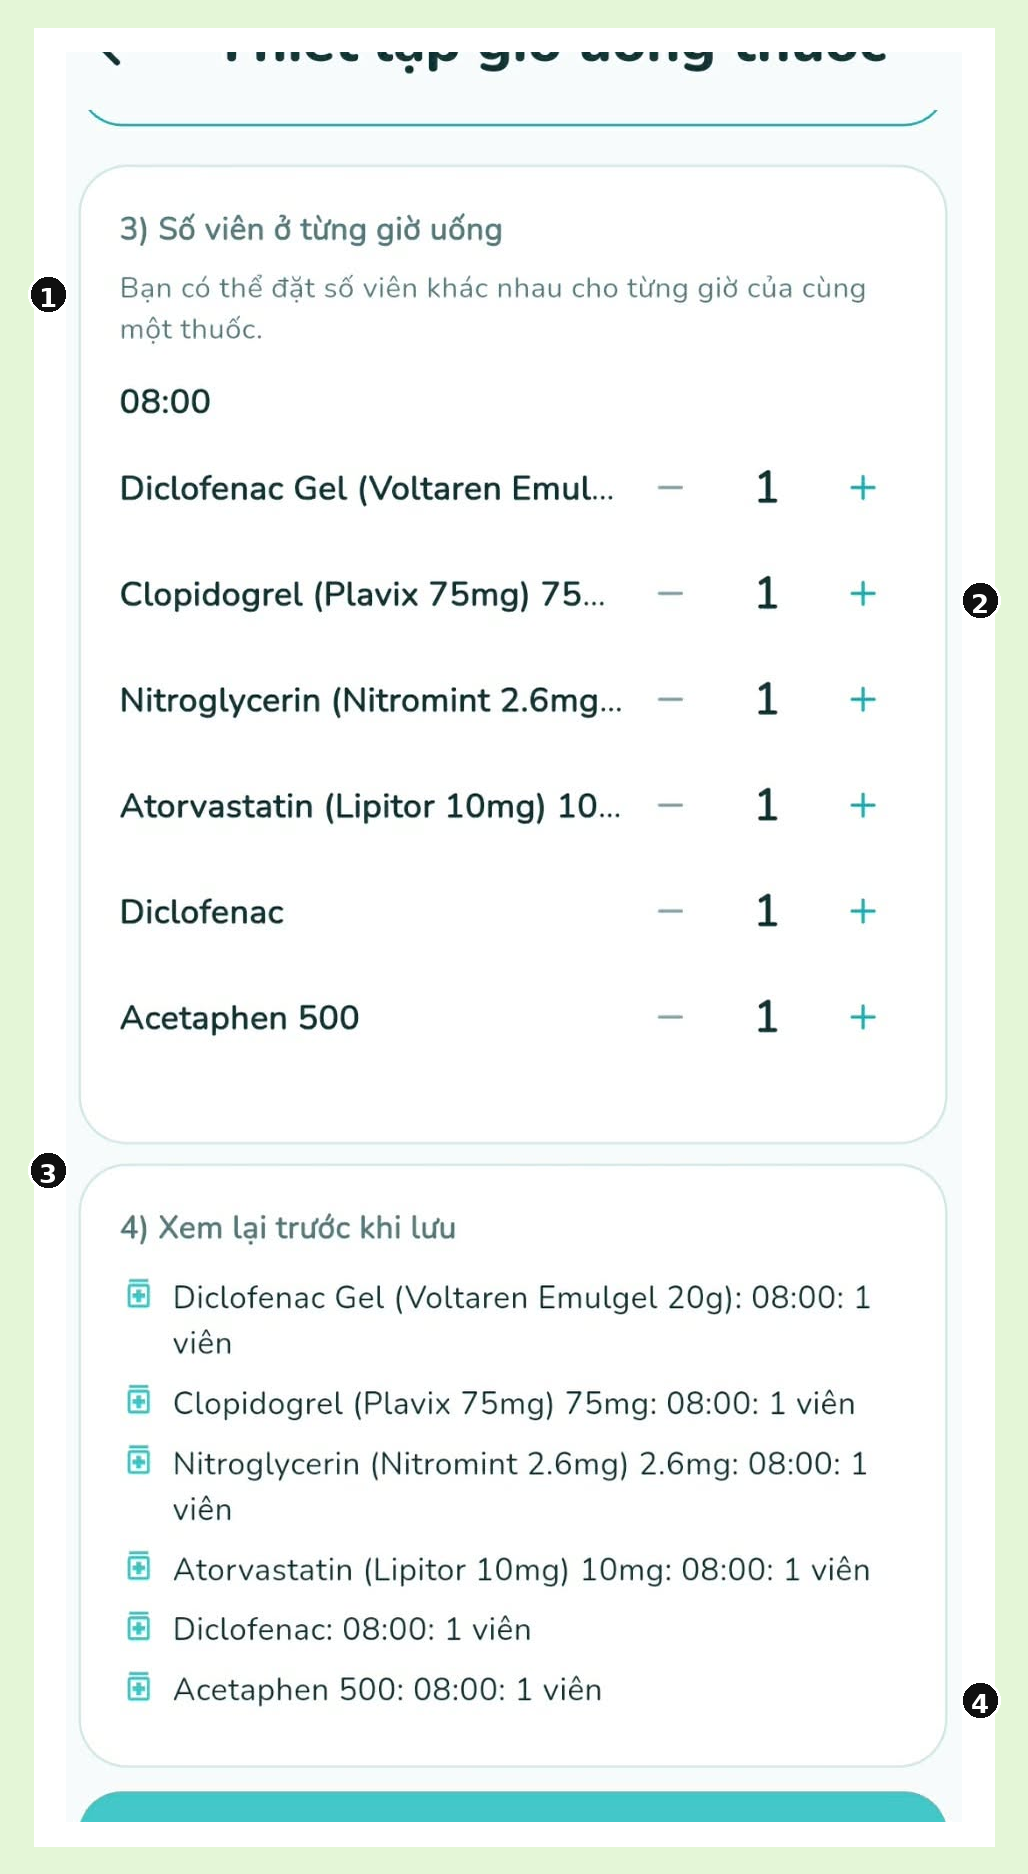
\includegraphics[width=0.52\textwidth]{assets/app/set_schedule_annotated.png}
\caption{Màn hình thiết lập lịch dùng thuốc (chọn khung giờ và số viên theo từng khung giờ)}
\label{fig:set-schedule}
\end{figure}

Các thành phần chính của màn hình thiết lập lịch được trình bày trong Bảng~\ref{tab:set-schedule-components}.

\begin{table}[H]
\centering
\caption{Các thành phần của màn hình thiết lập lịch dùng thuốc}
\label{tab:set-schedule-components}
{\renewcommand{\arraystretch}{1.35}
\begin{tabularx}{\textwidth}{J}
\TableHeader{\textbf{STT} & \textbf{Thành phần} & \textbf{Mô tả}}
\TableRow{1 & Phần mô tả bước hiện tại & Nhắc người dùng rằng đây là bước khai báo số viên cho từng khung giờ uống thuốc.}
\TableRow{2 & Bộ điều chỉnh số viên & Cho phép tăng hoặc giảm số viên của từng thuốc tại một khung giờ cụ thể.}
\TableRow{3 & Phần xem lại trước khi lưu & Tóm tắt cấu hình khung giờ và liều dùng để người dùng kiểm tra lần cuối.}
\TableRow{4 & Nút lưu kế hoạch & Gửi bản nháp lên máy chủ và kích hoạt bước tạo kế hoạch dùng thuốc chính thức.}
\end{tabularx}}
\end{table}

\section{Cài đặt chức năng theo dõi trong ngày}

\subsection{Giao diện theo dõi liều uống trong ngày}

Sau khi người dùng đã có kế hoạch dùng thuốc, ứng dụng hiển thị danh sách liều uống trong ngày từ API tổng hợp của máy chủ (Hình~\ref{fig:home-today}). Mỗi mục hiển thị giờ uống, tên thuốc, số viên và trạng thái hiện tại. Khi người dùng chọn ``Đã uống'' hoặc ``Bỏ qua'', ứng dụng gọi API ghi nhật ký tương ứng. Thiết kế này tạo thành một vòng kín giữa tạo kế hoạch, nhắc uống và theo dõi việc thực hiện.

\begin{figure}[H]
\centering
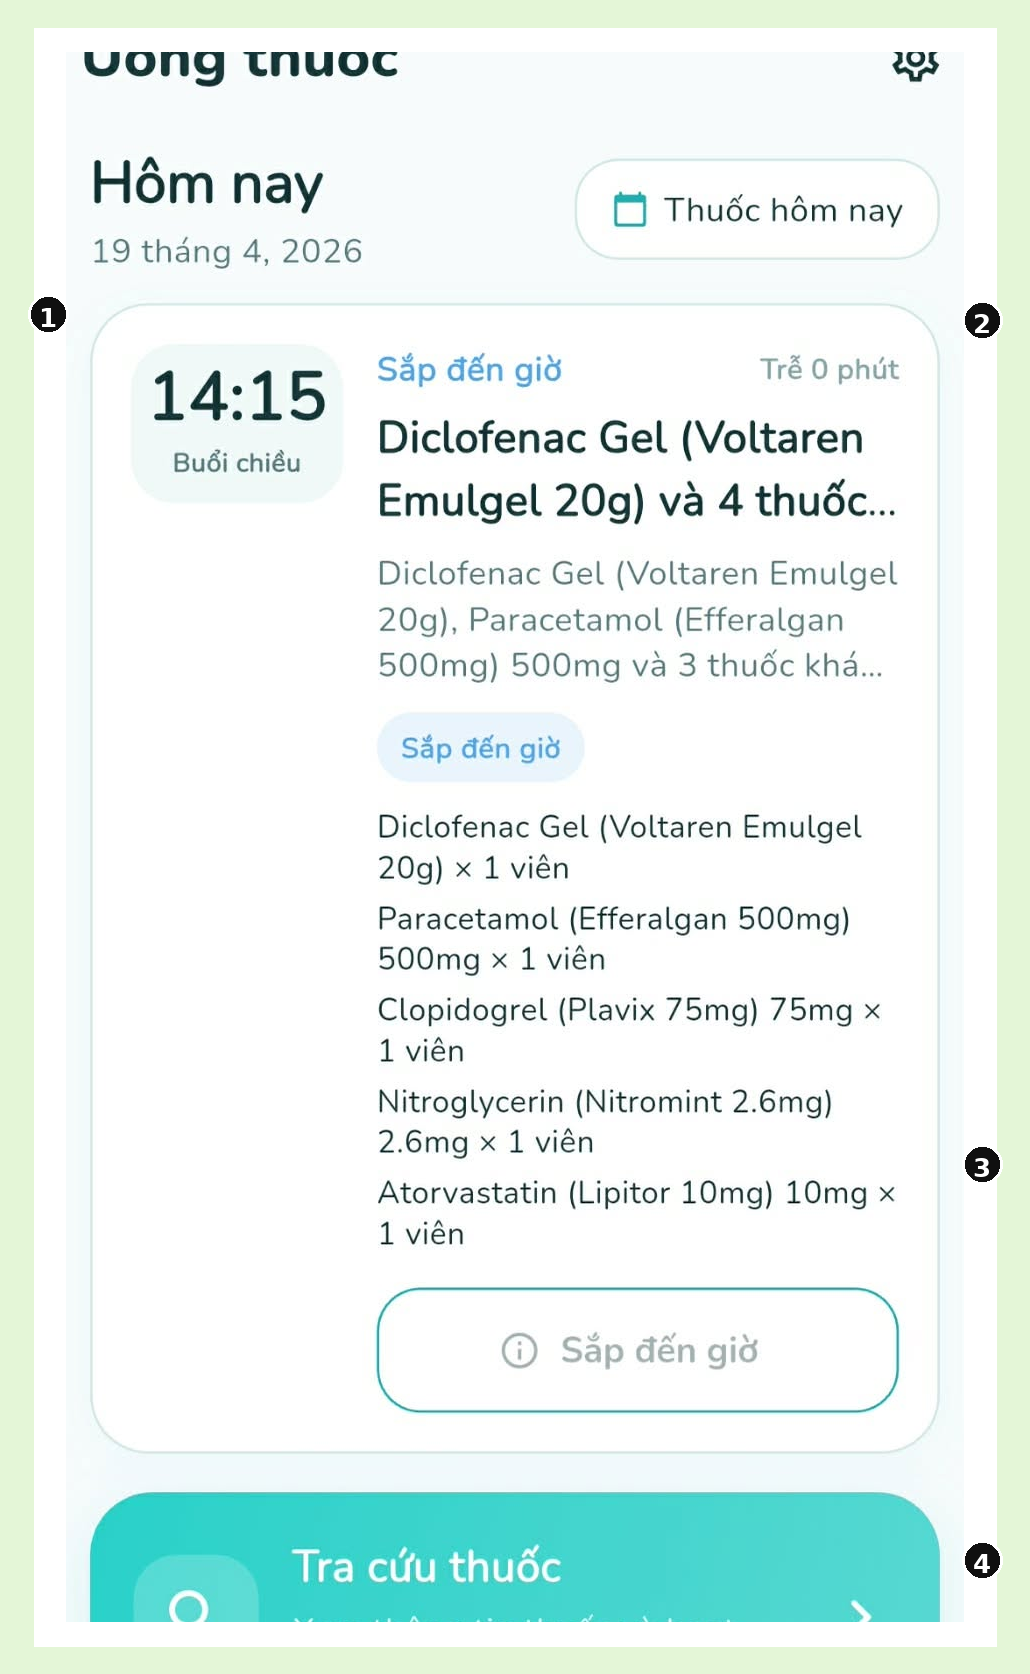
\includegraphics[width=0.52\textwidth]{assets/app/home_today_annotated.png}
\caption{Màn hình trang chủ hiển thị tóm tắt liều uống trong ngày và lịch tuần}
\label{fig:home-today}
\end{figure}

Trang chủ ứng dụng cung cấp một thẻ tóm tắt trực quan thể hiện tổng số liều cần dùng trong ngày, chia theo trạng thái đã uống, chờ, bỏ qua và quên. Phía dưới là thanh lịch tuần để người dùng nhanh chóng nhận ra hôm nay là ngày nào trong tuần. Cách trình bày này giúp người dùng theo dõi tiến độ dùng thuốc một cách trực quan mà không cần điều hướng qua nhiều màn hình.

Các thành phần chính của màn hình theo dõi trong ngày được trình bày trong Bảng~\ref{tab:home-today-components}.

\begin{table}[H]
\centering
\caption{Các thành phần của màn hình theo dõi trong ngày}
\label{tab:home-today-components}
{\renewcommand{\arraystretch}{1.35}
\begin{tabularx}{\textwidth}{J}
\TableHeader{\textbf{STT} & \textbf{Thành phần} & \textbf{Mô tả}}
\TableRow{1 & Thời điểm liều sắp đến giờ & Hiển thị khung giờ và buổi tương ứng của liều dùng gần nhất trong ngày.}
\TableRow{2 & Trạng thái thực hiện & Thể hiện mức độ trễ hoặc trạng thái hiện hành của liều dùng đang được theo dõi.}
\TableRow{3 & Danh sách thuốc trong liều & Tóm tắt các thuốc và số viên phải dùng trong khung giờ đang xét.}
\TableRow{4 & Thẻ điều hướng phụ trợ & Dẫn người dùng sang khu vực tra cứu thuốc, là chức năng hỗ trợ nằm ngoài luồng trung tâm của đề tài.}
\end{tabularx}}
\end{table}

\subsection{Giao diện lịch sử kế hoạch và nhật ký}

Ngoài màn hình theo dõi trong ngày, ứng dụng còn duy trì màn hình lịch sử kế hoạch và nhật ký dùng thuốc để người dùng xem lại tiến trình điều trị gần đây. Màn hình này đóng vai trò hỗ trợ, không phải trung tâm của đề tài, nhưng giúp hệ thống hoàn chỉnh hơn ở góc nhìn ứng dụng thực tế.

\begin{figure}[H]
\centering
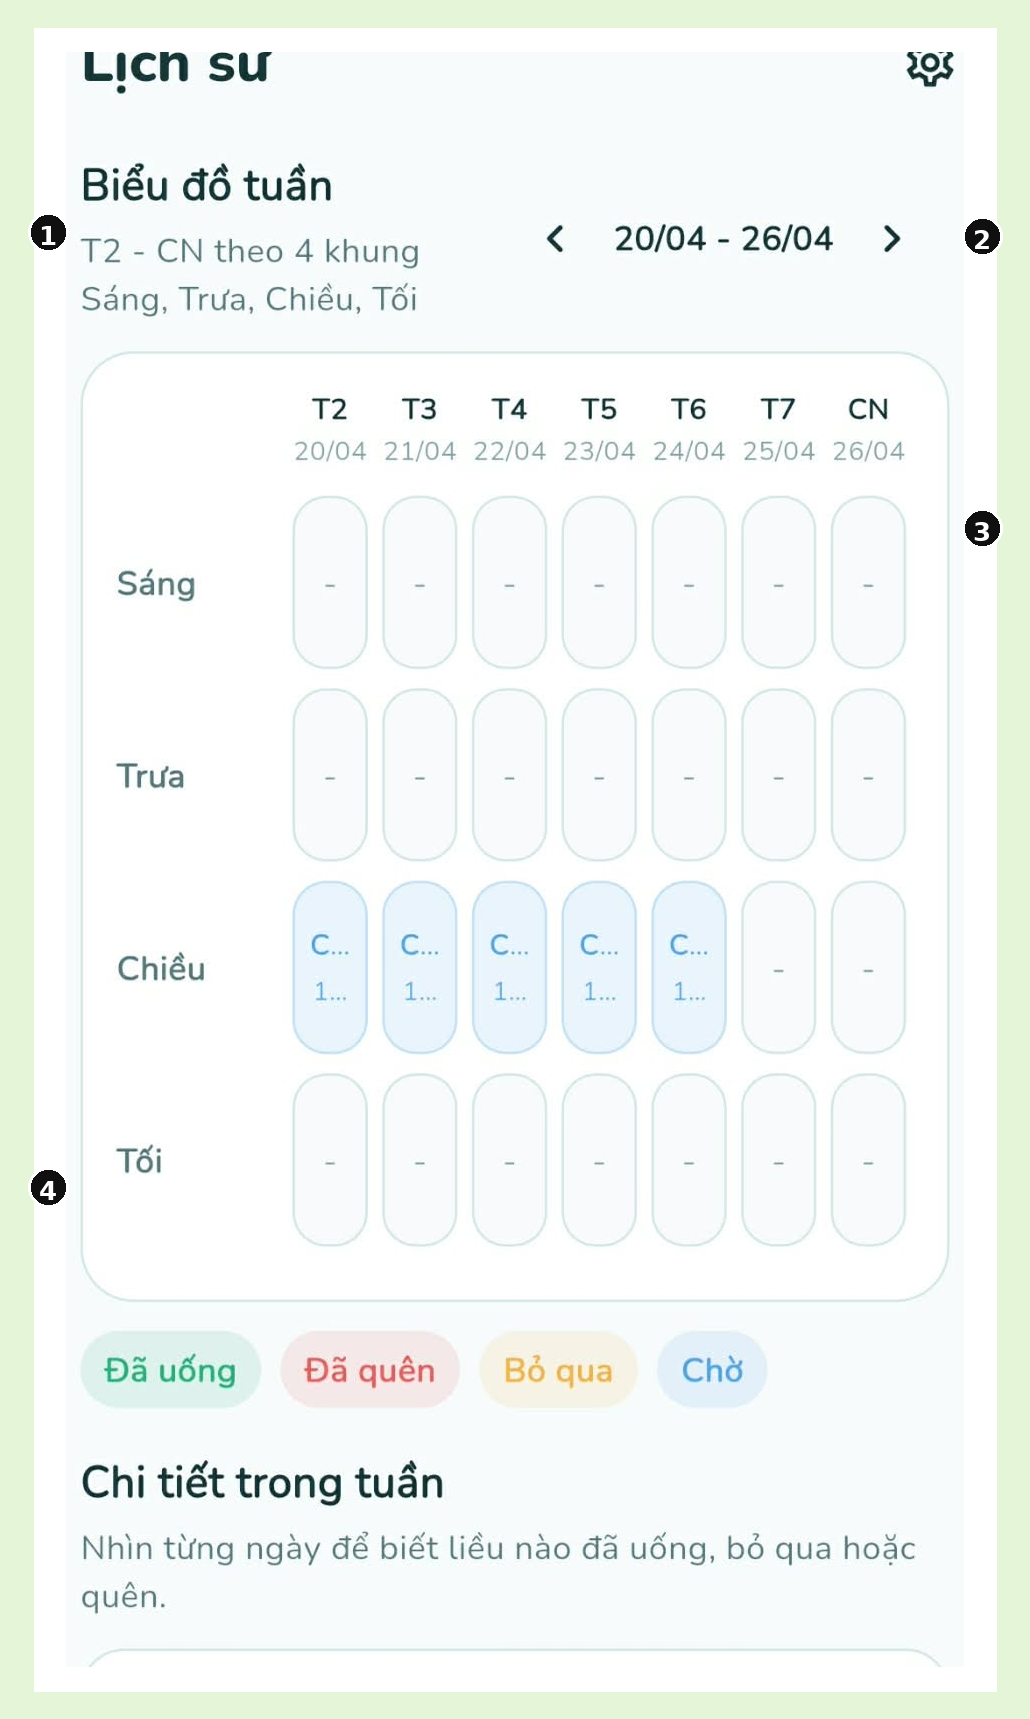
\includegraphics[width=0.52\textwidth]{assets/app/history_week_annotated.png}
\caption{Màn hình lịch sử kế hoạch và nhật ký dùng thuốc theo tuần}
\label{fig:history-week}
\end{figure}

Các thành phần chính của màn hình lịch sử được trình bày trong Bảng~\ref{tab:history-week-components}.

\begin{table}[H]
\centering
\caption{Các thành phần của màn hình lịch sử kế hoạch và nhật ký}
\label{tab:history-week-components}
{\renewcommand{\arraystretch}{1.35}
\begin{tabularx}{\textwidth}{J}
\TableHeader{\textbf{STT} & \textbf{Thành phần} & \textbf{Mô tả}}
\TableRow{1 & Tiêu đề và mô tả chu kỳ tuần & Xác định người dùng đang xem lịch sử theo chế độ tuần và theo bốn khung giờ trong ngày.}
\TableRow{2 & Bộ điều hướng tuần & Cho phép lùi hoặc tiến giữa các tuần để xem lại tiến trình điều trị.}
\TableRow{3 & Lưới trạng thái tuần & Hiển thị trạng thái từng khung giờ trong tuần để người dùng quan sát toàn cục.}
\TableRow{4 & Chú giải trạng thái & Diễn giải ý nghĩa các màu trạng thái như đã uống, quên, bỏ qua và chờ.}
\end{tabularx}}
\end{table}

\section{Một số quyết định cài đặt đáng chú ý}

\subsection{Tách máy chủ và mô-đun AI}

Nếu tích hợp trực tiếp toàn bộ trí tuệ nhân tạo vào máy chủ, dự án sẽ khó kiểm soát hơn ở cả mặt triển khai lẫn gỡ lỗi. Việc tách FastAPI thành một dịch vụ riêng giúp máy chủ tập trung vào xử lý nghiệp vụ và dữ liệu của ứng dụng, trong khi phần AI có thể được tối ưu theo nhịp riêng.

\subsection{Giữ bước rà soát thủ công sau AI}

Ứng dụng không coi kết quả của trí tuệ nhân tạo là dữ liệu cuối cùng. Thay vào đó, trí tuệ nhân tạo tạo ra danh sách thuốc sơ bộ và người dùng vẫn có bước rà soát trước khi lưu kế hoạch. Cách thiết kế này phù hợp hơn với ngữ cảnh y tế, nơi một sai sót nhỏ trong nhận diện thuốc có thể kéo theo hậu quả sử dụng sai thuốc hoặc sai liều.

\subsection{Biểu diễn liều dùng theo từng khung giờ}

Trong các phiên bản đầu, nhiều hệ thống thường chỉ lưu số viên chung cho một loại thuốc. Tuy nhiên, điều đó không phản ánh đúng thực tế sử dụng thuốc. Dự án hiện tại cài đặt mô hình liều dùng theo từng khung giờ, cho phép biểu diễn các trường hợp như sáng uống hai viên, tối uống một viên. Đây là một điểm cải thiện quan trọng ở tầng ứng dụng và máy chủ.

\chapter{THỰC NGHIỆM VÀ ĐÁNH GIÁ}

\section{Mục tiêu đánh giá}

Quá trình đánh giá trong đề tài tập trung vào ba mục tiêu. Thứ nhất là kiểm tra xem quy trình nhận diện đơn thuốc có đủ ổn định để tạo ra danh sách thuốc đủ sử dụng cho ứng dụng hay không. Thứ hai là kiểm tra xem luồng đầu cuối từ quét đơn đến tạo kế hoạch có vận hành được trong bối cảnh thực tế hay không. Thứ ba là đánh giá các giới hạn kỹ thuật của những chức năng mở rộng chưa được tích hợp.

\section{Dữ liệu và môi trường thử nghiệm}

Đề tài sử dụng tập ảnh đơn thuốc thực tế trong thư mục dữ liệu đầu vào nội bộ của dự án. Ở thời điểm tổng hợp báo cáo, dự án lưu tập ảnh đầu vào mẫu với 51 ảnh, trong khi một đợt benchmark nội bộ tiêu biểu của luồng nhận diện được ghi nhận trên 50 ảnh thực tế. Việc tách bạch như vậy nhằm tránh nhầm lẫn giữa toàn bộ tập input hiện có trong dự án và đúng tập ảnh đã được dùng để tổng hợp các số liệu benchmark trình bày ở phần sau. Ngoài ra, hệ thống còn được thử nghiệm theo luồng ứng dụng thực tế để kiểm tra khả năng tạo kế hoạch, nhắc uống và ghi nhận nhật ký dùng thuốc.

Các thử nghiệm được thực hiện trên môi trường có GPU RTX 3050 4GB để tận dụng khả năng tăng tốc cho nhận dạng ký tự quang học và nhận diện, đồng thời vẫn duy trì cơ chế chuyển sang CPU khi cần.

\section{Lưu ý về dữ liệu và quyền riêng tư}

Do ảnh đơn thuốc có thể chứa thông tin cá nhân của người bệnh, việc thu thập và sử dụng dữ liệu trong đề tài được xem xét theo hướng hạn chế tối đa rủi ro lộ lọt thông tin. Trong quá trình thử nghiệm và tổng hợp báo cáo, dữ liệu được dùng chủ yếu để đánh giá khả năng nhận diện thuốc và kiểm tra luồng hoạt động của hệ thống, không nhằm mục đích khai thác thông tin cá nhân ngoài phạm vi nghiên cứu.

Khi đưa dữ liệu vào báo cáo, đề tài ưu tiên trình bày kết quả ở dạng tổng hợp thay vì công bố trực tiếp toàn bộ nội dung đơn thuốc. Với các hình minh họa đã sử dụng trong báo cáo, các vùng có khả năng làm lộ thông tin cá nhân như họ tên, địa chỉ hoặc mã số khám bệnh tiếp tục được che hoặc lược bỏ.

\section{Tiêu chí đánh giá}

Để bảo đảm việc đánh giá bám sát mục tiêu thực tế của đề tài, các tiêu chí chính được sử dụng gồm:

\begin{enumerate}[label=\arabic*.]
    \item \textbf{Tỉ lệ xử lý thành công:} số ảnh được hệ thống xử lý hoàn chỉnh mà không phát sinh lỗi dừng xử lý.
    \item \textbf{Số lượng thuốc nhận diện được:} tổng số thuốc mà hệ thống trích xuất được từ tập ảnh thử nghiệm.
    \item \textbf{Khả năng sử dụng cho bước lập lịch:} mức độ mà danh sách thuốc đầu ra có thể được dùng trực tiếp hoặc chỉ cần chỉnh sửa nhỏ trước khi lập kế hoạch dùng thuốc.
    \item \textbf{Thời gian xử lý:} thời gian cần thiết để hệ thống trả về kết quả cho một ảnh đầu vào trong các trạng thái khởi động ban đầu và sau khi đã ổn định.
    \item \textbf{Tính hoàn chỉnh của luồng ứng dụng:} khả năng đi trọn từ quét đơn thuốc đến lưu kế hoạch và theo dõi việc dùng thuốc trong ngày.
\end{enumerate}

\section{Kết quả nhận diện đơn thuốc}

Theo một benchmark nội bộ tiêu biểu của dự án, quy trình nhận diện đơn thuốc đạt kết quả ổn định trên tập ảnh thực tế, với các chỉ số tổng hợp đáng chú ý như sau:

\begin{table}[htbp]
\centering
\caption{Snapshot kết quả benchmark nội bộ của quy trình nhận diện đơn thuốc}
\label{tab:phase-a-benchmark}
{\renewcommand{\arraystretch}{1.4}
\begin{tabularx}{\textwidth}{N}
\TableHeader{\textbf{STT} & \textbf{Chỉ số} & \textbf{Giá trị ghi nhận}}
\TableRow{1 & Số ảnh đánh giá chính & 50 ảnh đơn thuốc thực tế}
\TableRow{2 & Tỉ lệ xử lý thành công & 50/50 ảnh}
\TableRow{3 & Tổng số thuốc nhận được & 338 thuốc}
\TableRow{4 & Trung bình số thuốc trên mỗi ảnh & 6.8 thuốc/ảnh}
\TableRow{5 & Số lỗi hệ thống trong quá trình đánh giá thử nghiệm & 0 lỗi}
\TableRow{6 & Thời gian ảnh đầu tiên sau khi khởi động & khoảng 17 giây}
\TableRow{7 & Thời gian xử lý sau khi hệ thống đã ổn định & khoảng 7 giây/ảnh}
\end{tabularx}}
\end{table}

Một trường hợp điển hình được ghi nhận trong tài liệu kỹ thuật là ảnh đơn thuốc ở tập thử nghiệm \path{prescription_3/IMG_20260209_180505.jpg}, trong đó hệ thống nhận diện được đầy đủ 5/5 thuốc và đều tìm thấy kết quả trong cơ sở dữ liệu thuốc. Trường hợp này cho thấy khi chất lượng ảnh ở mức chấp nhận được và bố cục danh sách thuốc nằm trong phạm vi trí tuệ nhân tạo xử lý tốt, quy trình nhận diện có thể trả về kết quả đủ chất lượng để phục vụ luồng ứng dụng.

Góp phần mang lại thành công trên là khả năng khoanh vùng chính xác của bước phát hiện đa giác chữ thuộc PaddleOCR, được thể hiện thông qua Hình~\ref{fig:ocr-detection}. Hệ thống có khả năng đánh dấu các dòng dữ liệu riêng biệt không bị đứt quãng sai lệch bất chấp khoảng cách giữa các chữ số, từ ngữ.

\begin{figure}[tbp]
\centering
\includegraphics[width=0.7\textwidth]{assets/real_data/minhhoa.pdf}
\caption{Minh họa các đa giác phân định vùng văn bản được tìm thấy dựa trên ảnh đầu vào}
\label{fig:ocr-detection}
\end{figure}

Từ lượng thông tin này được trích xuất thành văn bản, các khối OCR thô sẽ lần lượt được tổng hợp và phân loại bằng mô hình học máy (PhoBERT NER) để cô lập được danh sách tên dược phẩm chính xác cho ứng dụng lập lịch dùng cuối cùng.

\section{Đánh giá hệ thống ứng dụng}

Ngoài quy trình xử lý trí tuệ nhân tạo, đề tài còn chú trọng kiểm tra tính hoàn chỉnh của hệ thống ở mức ứng dụng. Ở thời điểm hiện tại, repo duy trì các bộ kiểm thử tự động cho backend Node.js và pipeline Python, trong khi quy trình phát triển của phía di động còn bao gồm các bước kiểm tra như \texttt{flutter analyze} và \texttt{flutter test}. Do số lượng ca kiểm thử tiếp tục thay đổi theo tiến độ phát triển, báo cáo này ưu tiên nhấn mạnh sự hiện diện của test tự động thay vì giữ lại một con số pass snapshot dễ bị lỗi thời.

Xét trên khía cạnh luồng nghiệp vụ, hệ thống hiện đã hỗ trợ được chuỗi thao tác sau: quét đơn thuốc, rà soát kết quả nhận diện, lập lịch dùng thuốc, xem kế hoạch hôm nay, ghi nhận trạng thái dùng thuốc và xem lịch sử kế hoạch kèm nhật ký dùng thuốc. Điều này cho thấy đề tài không chỉ dừng ở mức thử nghiệm trí tuệ nhân tạo độc lập mà đã tiến tới một hệ thống phần mềm có giá trị sử dụng thực tế.

\section{Các dạng sai sót điển hình}

Trong quá trình thử nghiệm, một số dạng sai sót điển hình có thể ảnh hưởng đến kết quả nhận diện đã được ghi nhận. Thứ nhất là ảnh bị nghiêng, mờ hoặc chói sáng, làm giảm khả năng phát hiện vùng chữ và kéo theo sai số ở bước nhận dạng ký tự. Thứ hai là bố cục đơn thuốc không đồng đều, khiến một số khối chữ khó được gom đúng ngữ cảnh. Thứ ba là tên thuốc bị viết tắt, in mờ hoặc nằm gần các dòng hướng dẫn dùng thuốc, dẫn đến nguy cơ trích xuất nhầm hoặc thiếu.

Các dạng sai sót này cho thấy chất lượng đầu vào vẫn là yếu tố ảnh hưởng rất mạnh đến độ ổn định của hệ thống. Vì vậy, việc giữ bước rà soát thủ công ở phía người dùng tiếp tục là một quyết định phù hợp trong phiên bản hiện tại.

\section{Ưu điểm của hệ thống}

Các ưu điểm chính của hệ thống gồm:

\begin{itemize}[leftmargin=1.5cm]
    \item Có luồng hoạt động đầu cuối rõ ràng từ ảnh đơn thuốc đến kế hoạch dùng thuốc.
    \item Kết hợp trí tuệ nhân tạo theo hướng hỗ trợ người dùng, không loại bỏ hoàn toàn vai trò rà soát thủ công.
    \item Kiến trúc tách lớp giúp dễ bảo trì và dễ mở rộng.
    \item Phần lịch dùng thuốc phản ánh tương đối sát nhu cầu thực tế nhờ hỗ trợ số viên theo từng khung giờ.
    \item Có lưu lịch sử và trạng thái dùng thuốc, tạo nền tảng cho các phân tích sâu hơn trong tương lai.
\end{itemize}

\section{Hạn chế của hệ thống}

Mặc dù đạt được kết quả khả quan ở luồng chính, hệ thống vẫn còn một số hạn chế:

\begin{itemize}[leftmargin=1.5cm]
    \item Độ chính xác của bước nhận dạng ký tự quang học vẫn chịu ảnh hưởng mạnh bởi chất lượng ảnh chụp đầu vào.
    \item Dữ liệu quét đơn thuốc thực tế rất đa dạng nên khó đảm bảo một mức độ ổn định tuyệt đối cho mọi loại đơn.
    \item Kết quả chuẩn hóa tên thuốc phụ thuộc vào dữ liệu thuốc nội bộ và chất lượng đối sánh gần đúng.
    \item Mặc dù repo hiện đã có một số thành phần thử nghiệm cho bài toán xác minh viên thuốc, chức năng này vẫn chưa đạt ngưỡng phù hợp để đưa vào luồng chính đã được đánh giá.
\end{itemize}

\section{Vì sao chưa mở rộng nhận dạng ký tự quang học sang toàn bộ thông tin trên đơn thuốc}

Trong quá trình phát triển, đề tài có cân nhắc khả năng trích xuất thêm các trường thông tin như họ tên bệnh nhân, triệu chứng hoặc chẩn đoán. Tuy nhiên, việc mở rộng này chưa được tích hợp vào phiên bản chính vì ba lý do.

Thứ nhất, các trường thông tin ngoài danh sách thuốc thường có vị trí và bố cục kém ổn định hơn. Không giống danh sách thuốc vốn thường nằm trong khu vực bảng kê hoặc vùng nội dung chính, các vùng như chẩn đoán hoặc ghi chú có thể ngắn, nhỏ, đặt ở nhiều vị trí khác nhau và dễ bị che khuất hoặc mờ.

Thứ hai, mở rộng phạm vi nhận dạng ký tự quang học đồng nghĩa với việc hệ thống phải đọc nhiều vùng hơn, nhiều khối chữ hơn và xử lý thêm nhiều tình huống nhiễu hơn. Điều đó làm tăng thời gian xử lý tổng thể. Trong bối cảnh người dùng di động mong muốn quét nhanh để lập lịch dùng thuốc, việc tăng thêm độ trễ chỉ để lấy các trường chưa phục vụ trực tiếp cho luồng chính là một đánh đổi chưa tối ưu.

Thứ ba, khi muốn lấy thêm những trường thông tin này, ảnh đầu vào phải được chụp đầy đủ hơn, ít cắt mép hơn, thẳng góc hơn và rõ nét hơn. Nói cách khác, yêu cầu đặt lên người dùng sẽ cao hơn. Trong khi mục tiêu trải nghiệm người dùng của đề tài là giảm gánh nặng thao tác cho người dùng, đặc biệt là người lớn tuổi, việc buộc họ phải chụp ảnh quá chuẩn là không phù hợp với định hướng sản phẩm hiện tại.

Từ các lý do trên, đề tài chủ động giới hạn phạm vi nhận dạng ký tự quang học ở các thông tin phục vụ trực tiếp cho bài toán nhận diện thuốc và tạo kế hoạch dùng thuốc.

\section{Giới hạn của số liệu thử nghiệm}

Các số liệu trình bày trong báo cáo là kết quả đánh giá thử nghiệm nội bộ trong phạm vi phát triển của đề tài. Những số liệu này có giá trị phản ánh mức độ hoàn thiện kỹ thuật của hệ thống ở giai đoạn hiện tại, nhưng chưa nên được xem là kết luận cuối cùng cho mọi bối cảnh sử dụng thực tế.

Nguyên nhân là bộ dữ liệu thử nghiệm vẫn chủ yếu nằm trong phạm vi ảnh đơn thuốc thu thập được trong quá trình phát triển. Môi trường thử nghiệm phần lớn được thực hiện trên cấu hình phần cứng cố định của dự án. Vì vậy, nếu triển khai trên tập dữ liệu lớn hơn, đa dạng hơn hoặc trong môi trường thiết bị khác, kết quả có thể thay đổi.

Một giới hạn quan trọng cần làm rõ là đánh giá hiện tại chưa bao gồm các chỉ số độ chính xác và độ bao phủ ở mức toàn bộ quy trình nhận diện. Báo cáo chỉ ghi nhận tỉ lệ xử lý thành công, tổng số thuốc trích xuất được và thời gian xử lý. Việc tính các chỉ số này đòi hỏi phải có tập dữ liệu kiểm thử có nhãn thủ công với danh sách thuốc chuẩn cho từng ảnh, điều mà đề tài chưa thực hiện được trong phạm vi thời gian hiện tại. Do đó, chưa thể kết luận định lượng về tỉ lệ nhận diện đúng hoặc tỉ lệ bỏ sót tên thuốc trên toàn bộ quy trình. Đây là hướng cần bổ sung trong các đợt đánh giá tiếp theo nếu muốn nâng cao tiêu chuẩn học thuật của hệ thống.

\section{Vì sao chưa tích hợp chức năng xác minh viên thuốc qua hình ảnh}

Một hướng mở rộng khác của đề tài là xây dựng chức năng xác minh viên thuốc qua hình ảnh. Ở trạng thái hiện tại của dự án, hướng này đã có đường dẫn API và màn hình thử nghiệm riêng, nhưng chúng chưa được xem là một phần của luồng trung tâm đã được kiểm chứng trong báo cáo. Lý do cốt lõi là bài toán này có rủi ro an toàn cao nếu chưa đạt độ tin cậy đủ mạnh.

Trong thực tế, nhiều viên thuốc có ngoại hình rất giống nhau, đặc biệt là các viên nén tròn màu trắng. Theo hướng dẫn hình ảnh SPL của DailyMed, ảnh tham chiếu muốn hữu ích cho nhận diện phải thể hiện rõ cả mặt trước, mặt sau, dấu in, ký hiệu, vạch chia và màu sắc của viên thuốc \cite{dailymed-spl}. Nếu người dùng chỉ chụp một mặt hoặc chụp trong điều kiện ảnh không đủ tốt, hệ thống rất dễ nhầm lẫn giữa các viên có hình dạng gần tương tự nhau. Một nghiên cứu về nhận diện viên thuốc bằng học sâu cũng cho thấy các lớp khó nhất thường rơi vào nhóm viên trắng, tròn hoặc gần như chỉ khác nhau ở dấu khắc rất khó đọc \cite{pill-ai}.

Một vấn đề khác là cùng một hoạt chất có thể có ngoại hình khác nhau giữa các nhà sản xuất. Theo FDA, thuốc generic có thể khác về thành phần tá dược như màu sắc hoặc hương liệu, từ đó dẫn đến khác biệt về hình thức bên ngoài \cite{fda-generic}. Điều này khiến việc suy ra một "ngoại hình chuẩn" từ tên thuốc trở nên không đáng tin cậy nếu không có bộ dữ liệu tham chiếu rất chặt chẽ theo từng hãng, từng hàm lượng và từng dạng bào chế \cite{generic-appearance}. Từ góc nhìn an toàn sử dụng thuốc, MedlinePlus cũng nhấn mạnh rằng việc dùng nhầm thuốc hoặc dùng sai liều có thể gây hậu quả nghiêm trọng \cite{medlineplus-safety}.

Vì vậy, dù hướng xác minh viên thuốc qua hình ảnh là một hướng nghiên cứu có giá trị, báo cáo này chỉ xem đó là hướng mở rộng đang ở trạng thái thử nghiệm, chưa đủ an toàn để được gộp vào luồng chính đã được đánh giá. Các nguyên nhân chính gồm:

\begin{enumerate}[label=\arabic*.]
    \item Nhiều viên thuốc có ngoại hình thị giác quá giống nhau.
    \item Dấu in là tín hiệu phân biệt quan trọng nhưng khó chụp ổn định trong điều kiện sử dụng thực tế.
    \item Cùng một hoạt chất có thể có nhiều ngoại hình khác nhau giữa các nhà sản xuất.
    \item Việc yêu cầu người dùng chụp đủ hai mặt, đủ sáng, đúng góc làm tăng gánh nặng thao tác và giảm tính thực dụng của sản phẩm.
    \item Sai sót ở bước xác minh viên thuốc có thể kéo theo rủi ro an toàn cao hơn nhiều so với sai sót ở bước gợi ý kết quả nhận dạng ký tự.
\end{enumerate}

\chapter{KẾT LUẬN VÀ HƯỚNG PHÁT TRIỂN}

\section{Kết luận}

Đề tài đã hoàn thiện và kiểm thử một hệ thống hỗ trợ quét đơn thuốc và lập kế hoạch dùng thuốc, bao gồm luồng đầu cuối từ ảnh đơn thuốc giấy đến kế hoạch dùng thuốc trên ứng dụng di động.

Về kiến trúc, hệ thống gồm ba thành phần tách biệt: ứng dụng di động Flutter xử lý giao diện người dùng, máy chủ Node.js quản lý nghiệp vụ và dữ liệu với PostgreSQL, và dịch vụ AI bằng FastAPI thực hiện chuỗi nhận diện đơn thuốc. Chuỗi xử lý AI được chia thành các bước rõ ràng gồm phát hiện vùng đơn thuốc bằng YOLO, tiền xử lý ảnh, OCR kết hợp PaddleOCR và VietOCR, trích xuất tên thuốc bằng PhoBERT NER và đối sánh cơ sở dữ liệu thuốc Việt Nam. Thiết kế hệ thống đặt bước rà soát thủ công của người dùng làm bắt buộc trước khi tạo kế hoạch, nhằm giảm rủi ro trong bối cảnh ứng dụng y tế.

Một benchmark snapshot nội bộ trên 50 ảnh đơn thuốc thực tế cho thấy hệ thống đạt tỉ lệ xử lý thành công 100\%, không phát sinh lỗi dừng xử lý, và trung bình nhận diện 6,8 thuốc trên mỗi ảnh. Luồng ứng dụng từ quét đơn đến lưu kế hoạch và theo dõi uống thuốc đã hoạt động hoàn chỉnh. Ở mặt kỹ thuật phần mềm, phía máy chủ và pipeline Python đều được bao phủ bởi các bộ kiểm thử tự động đang tiếp tục được mở rộng theo tiến độ phát triển. Những kết quả này cho thấy hệ thống đáp ứng được các mục tiêu ban đầu ở mức thực nghiệm nội bộ.

\section{Những nội dung chưa nằm trong phạm vi đánh giá trung tâm}

Trong quá trình thực hiện, đề tài có xem xét một số hướng mở rộng như trích xuất thêm thông tin bệnh nhân, triệu chứng, chẩn đoán và xác minh viên thuốc qua hình ảnh. Một phần trong số đó hiện đã có thành phần ở mức route, màn hình hoặc bảng dữ liệu trong dự án. Tuy nhiên, thay vì đưa tất cả vào phần đánh giá trung tâm, đề tài chọn cách thu hẹp phạm vi để bảo toàn tính ổn định và tính thực dụng của luồng chính.

Việc chưa đưa các hướng này vào sản phẩm chính không nên được xem là thất bại của đề tài, mà là một quyết định kỹ thuật có chủ đích. Trong bối cảnh đề tài, việc lựa chọn một phạm vi phù hợp, làm rõ giới hạn và đánh giá trung thực các rủi ro là cần thiết hơn so với việc cố đưa vào các chức năng chưa đạt ngưỡng chất lượng sử dụng thực tế.

\section{Hướng phát triển trong tương lai}

Từ kết quả hiện tại, đề tài có thể được mở rộng theo một số hướng sau:

\begin{enumerate}[label=\arabic*.]
    \item \textbf{Mở rộng nhận dạng ký tự theo vùng thông minh:} thay vì nhận dạng toàn bộ đơn thuốc một cách đồng loạt, có thể nghiên cứu phát hiện riêng từng vùng như thông tin bệnh nhân, chẩn đoán hoặc hướng dẫn để giảm chi phí xử lý và tăng độ chính xác.
    \item \textbf{Nâng cấp dữ liệu thuốc và chuẩn hóa sâu hơn:} cải thiện cơ sở dữ liệu thuốc, tăng khả năng đối sánh giữa tên thương mại và hoạt chất, đồng thời bổ sung các thông tin bổ sung hữu ích cho bước rà soát.
    \item \textbf{Cải thiện chức năng xác minh viên thuốc:} nếu tiếp tục nghiên cứu hướng này, cần có chiến lược thu thập ảnh tham chiếu chuẩn hơn, ưu tiên nhận diện dấu in trên viên thuốc, chụp đủ hai mặt và đánh giá an toàn nghiêm ngặt trước khi đưa vào luồng chính.
    \item \textbf{Mở rộng đồng bộ và quản lý người dùng:} phát triển thêm các chức năng đồng bộ dữ liệu nhiều thiết bị, quản lý nhiều người dùng hoặc quản lý thuốc cho thành viên gia đình.
    \item \textbf{Đánh giá người dùng thực tế:} tổ chức khảo sát hoặc thử nghiệm người dùng, đặc biệt với người lớn tuổi, để đo mức độ dễ sử dụng của luồng quét đơn và lập lịch dùng thuốc.
\end{enumerate}

\section{Tổng kết cuối cùng}

Nhìn chung, đề tài cho thấy một hướng tiếp cận phù hợp cho bài toán số hóa đơn thuốc trong bối cảnh ứng dụng di động: không đặt toàn bộ kỳ vọng vào mô hình trí tuệ nhân tạo, mà kết hợp trí tuệ nhân tạo với thiết kế hệ thống và trải nghiệm người dùng để tạo ra giá trị sử dụng thực tế. Điểm cốt lõi của hệ thống là trí tuệ nhân tạo hỗ trợ người dùng ra quyết định tốt hơn, chứ không thay thế hoàn toàn người dùng trong các tình huống có độ nhạy cao liên quan đến việc sử dụng thuốc.

\clearpage

\begingroup
\sloppy
\raggedright
\phantomsection
\addcontentsline{toc}{chapter}{TÀI LIỆU THAM KHẢO}
\begin{thebibliography}{99}

\bibitem{paddleocr}
PaddlePaddle Authors, "PaddleOCR: Awesome multilingual OCR toolkits and benchmark." [Trực tuyến]. Có tại: \url{https://github.com/PaddlePaddle/PaddleOCR}. [Truy cập: Tháng 4 năm 2026].

\bibitem{vietocr}
P. Q. Nguyen, "VietOCR: Vietnamese OCR toolkit." [Trực tuyến]. Có tại: \url{https://github.com/pbcquoc/vietocr}. [Truy cập: Tháng 4 năm 2026].

\bibitem{phobert}
D. Q. Nguyen và A. T. Nguyen, "PhoBERT: Pre-trained language models for Vietnamese," trong \textit{Findings of the Association for Computational Linguistics: EMNLP 2020}, 2020, tr. 1037--1042.

\bibitem{dailymed-spl}
National Library of Medicine, "DailyMed SPL Image Guidelines." [Trực tuyến]. Có tại: \url{https://dailymed.nlm.nih.gov/dailymed/splimage-guidelines.cfm}. [Truy cập: Tháng 4 năm 2026].

\bibitem{pill-ai}
M. A. Zunair và cộng sự, "Pill Image Recognition for Medication Safety using Deep Learning." [Trực tuyến]. Có tại: \url{https://pmc.ncbi.nlm.nih.gov/articles/PMC6550183/}. [Truy cập: Tháng 4 năm 2026].

\bibitem{fda-generic}
U.S. Food and Drug Administration, "Generic Drugs Undergo Rigorous FDA Review." [Trực tuyến]. Có tại: \url{https://www.fda.gov/consumers/consumer-updates/generic-drugs-undergo-rigorous-fda-review}. [Truy cập: Tháng 4 năm 2026].

\bibitem{generic-appearance}
K. Kesselheim và cộng sự, "Patient views about generic medication appearance changes," \textit{Annals of Internal Medicine}, 2019. [Trực tuyến]. Có tại: \url{https://pmc.ncbi.nlm.nih.gov/articles/PMC6420535/}. [Truy cập: Tháng 4 năm 2026].

\bibitem{medlineplus-safety}
MedlinePlus, "Medicine safety - Filling your prescription." [Trực tuyến]. Có tại: \url{https://medlineplus.gov/ency/patientinstructions/000766.htm}. [Truy cập: Tháng 4 năm 2026].

\bibitem{yolo}
J. Redmon và cộng sự, "You Only Look Once: Unified, Real-Time Object Detection," trong \textit{Proceedings of the IEEE Conference on Computer Vision and Pattern Recognition (CVPR)}, 2016, tr. 779--788.

\bibitem{flutter}
Flutter Team, "Flutter documentation." [Trực tuyến]. Có tại: \url{https://docs.flutter.dev/}. [Truy cập: Tháng 4 năm 2026].

\bibitem{postgresql}
PostgreSQL Global Development Group, "PostgreSQL documentation." [Trực tuyến]. Có tại: \url{https://www.postgresql.org/docs/}. [Truy cập: Tháng 4 năm 2026].

\bibitem{fastapi}
S. Ramirez, "FastAPI documentation." [Trực tuyến]. Có tại: \url{https://fastapi.tiangolo.com/}. [Truy cập: Tháng 4 năm 2026].

\bibitem{express}
Express.js, "Express web framework." [Trực tuyến]. Có tại: \url{https://expressjs.com/}. [Truy cập: Tháng 4 năm 2026].

\end{thebibliography}
\endgroup

\end{document}
